\documentclass[../Dore_vision.tex]{subfiles}

\begin{document}

\section{Canto 03}

\begin{figure}[ht]
\centering
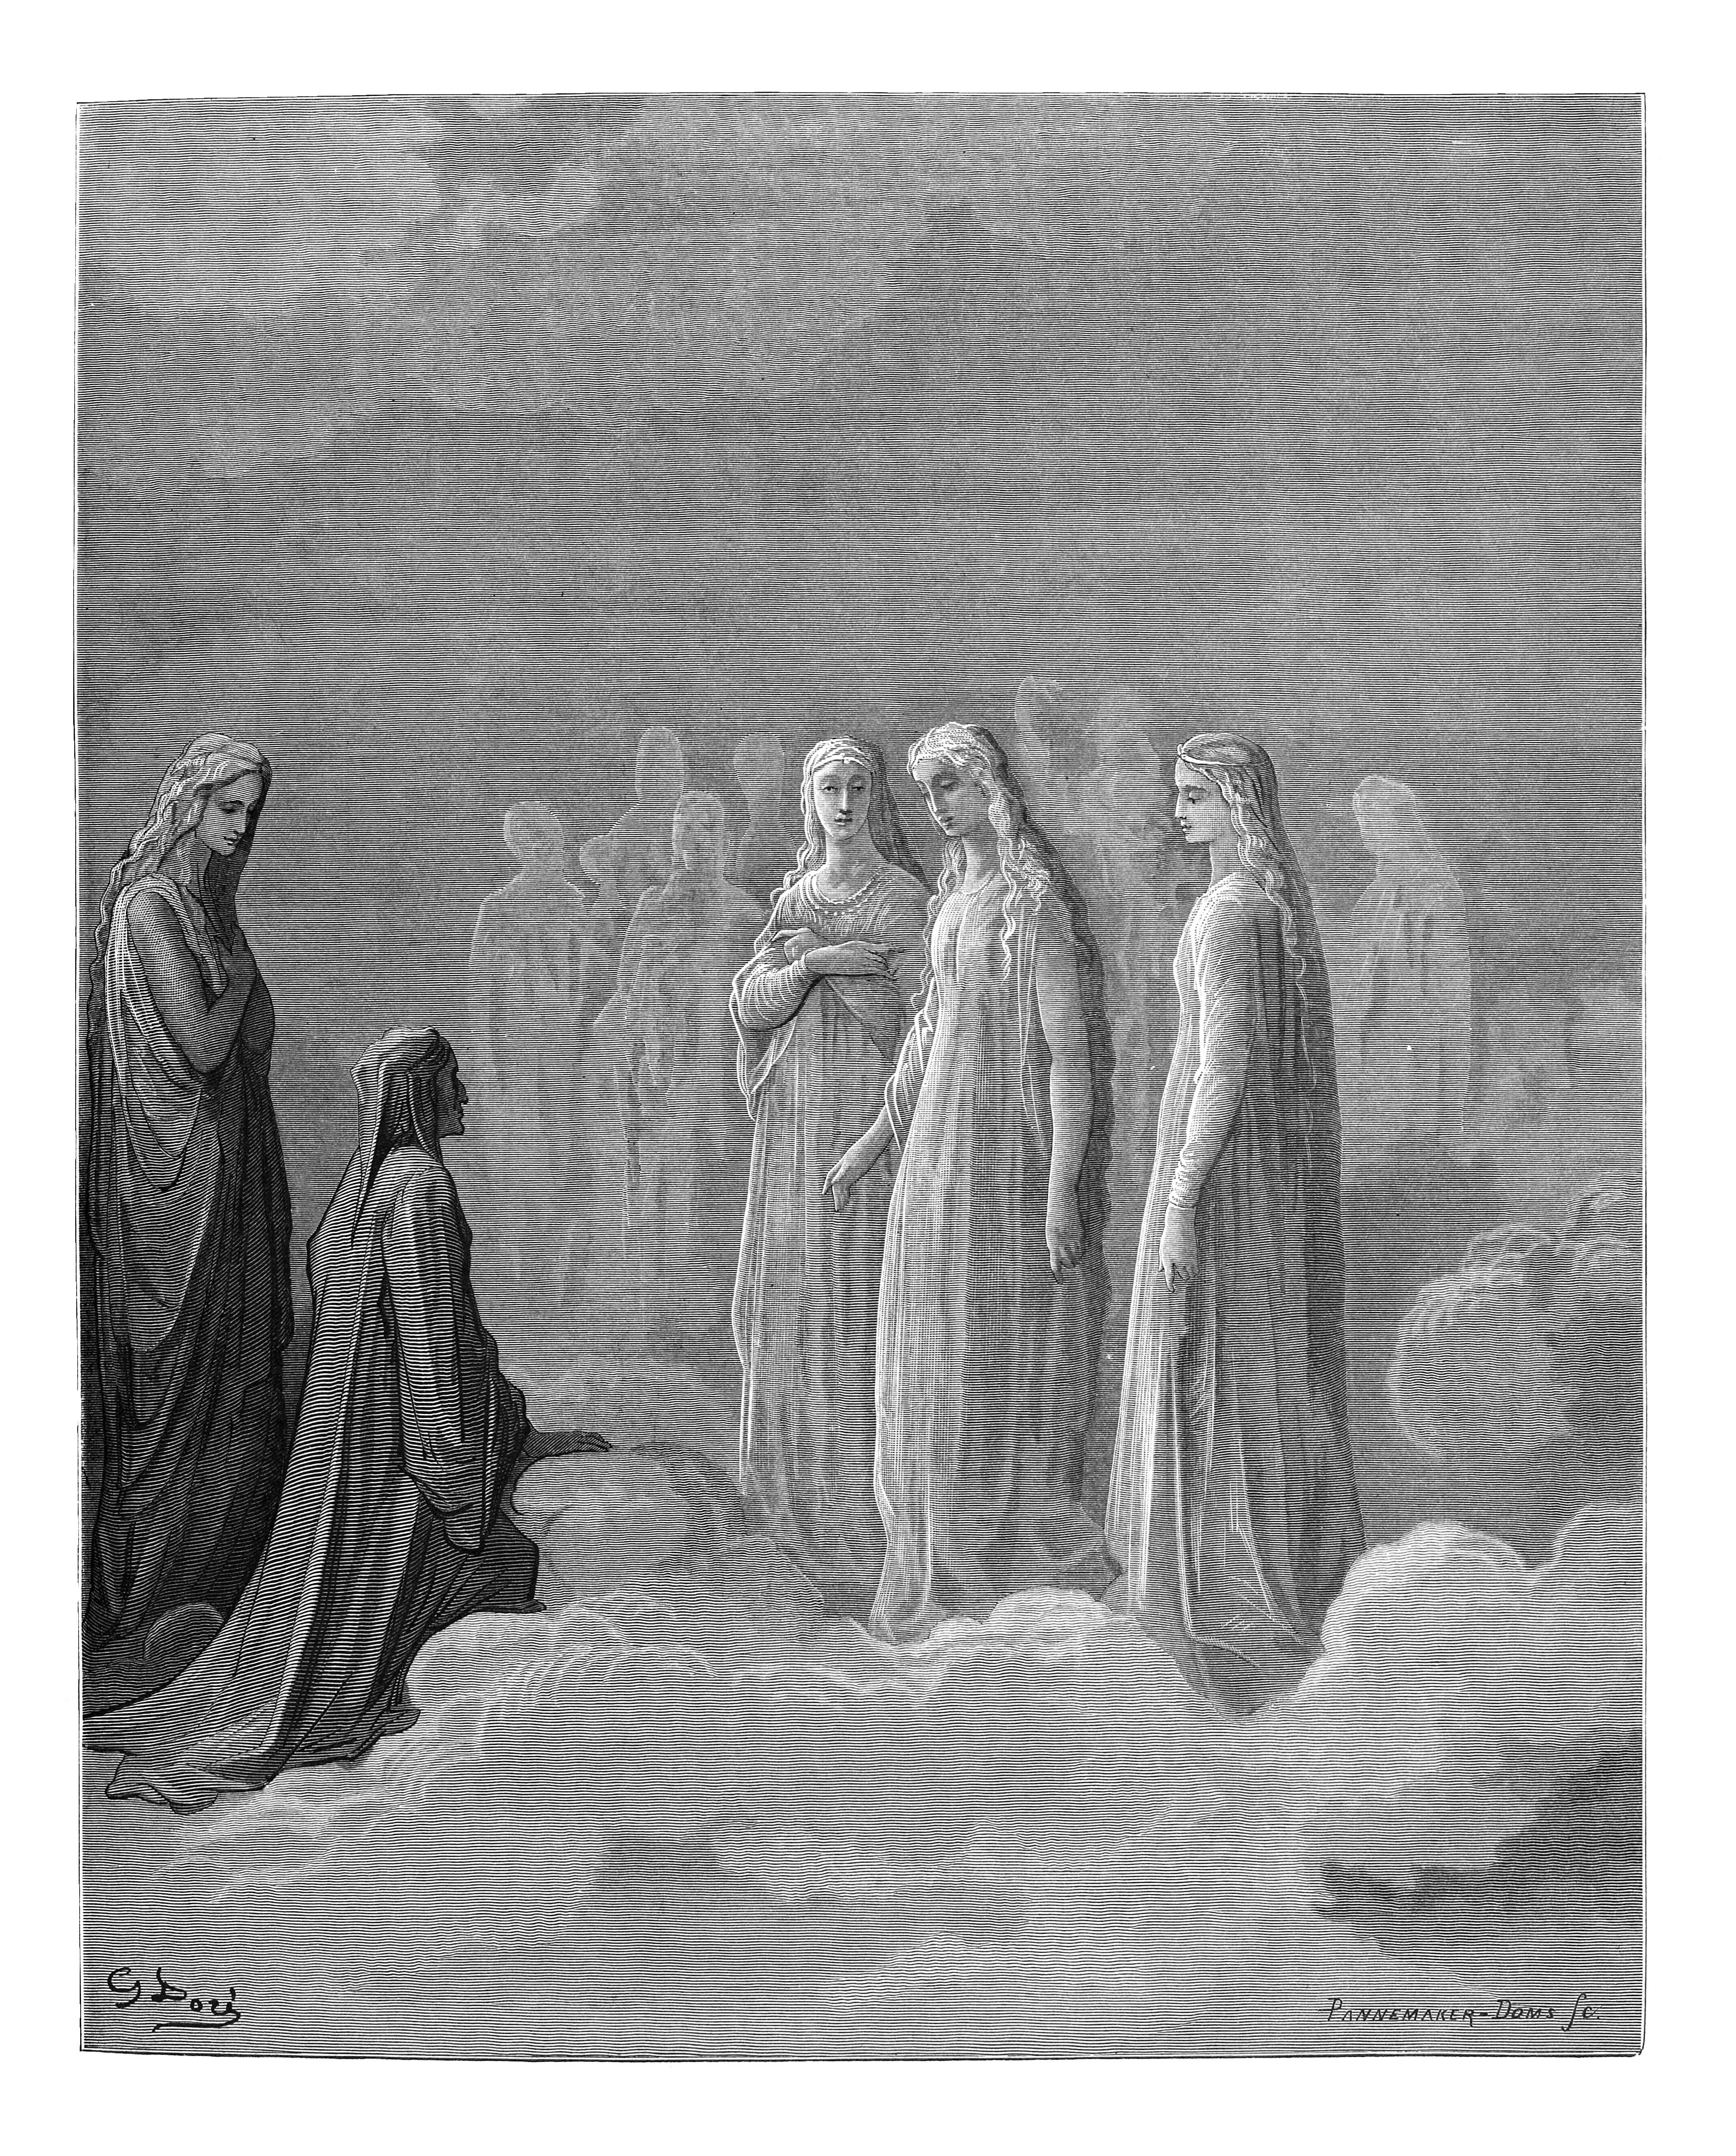
\includegraphics[height=\figsize]{illustrations/book_3/V03, c03.jpg}
\end{figure}

\begin{center}
\begin{minipage}{0.8\linewidth}
\textit{\\
"...se la mente tua ben sé riguarda,\\non mi ti celerà l’esser più bella,"} \\
—V03, c03 \\~\\
\textit{"...if thy mind observe me well, this form,\\With such addition grac'd of loveliness,\\Will not conceal me long, …"} \\
—B03, c03
\end{minipage}
\end{center}

\newpage

\section{Canto 05}

\begin{figure}[ht]
\centering
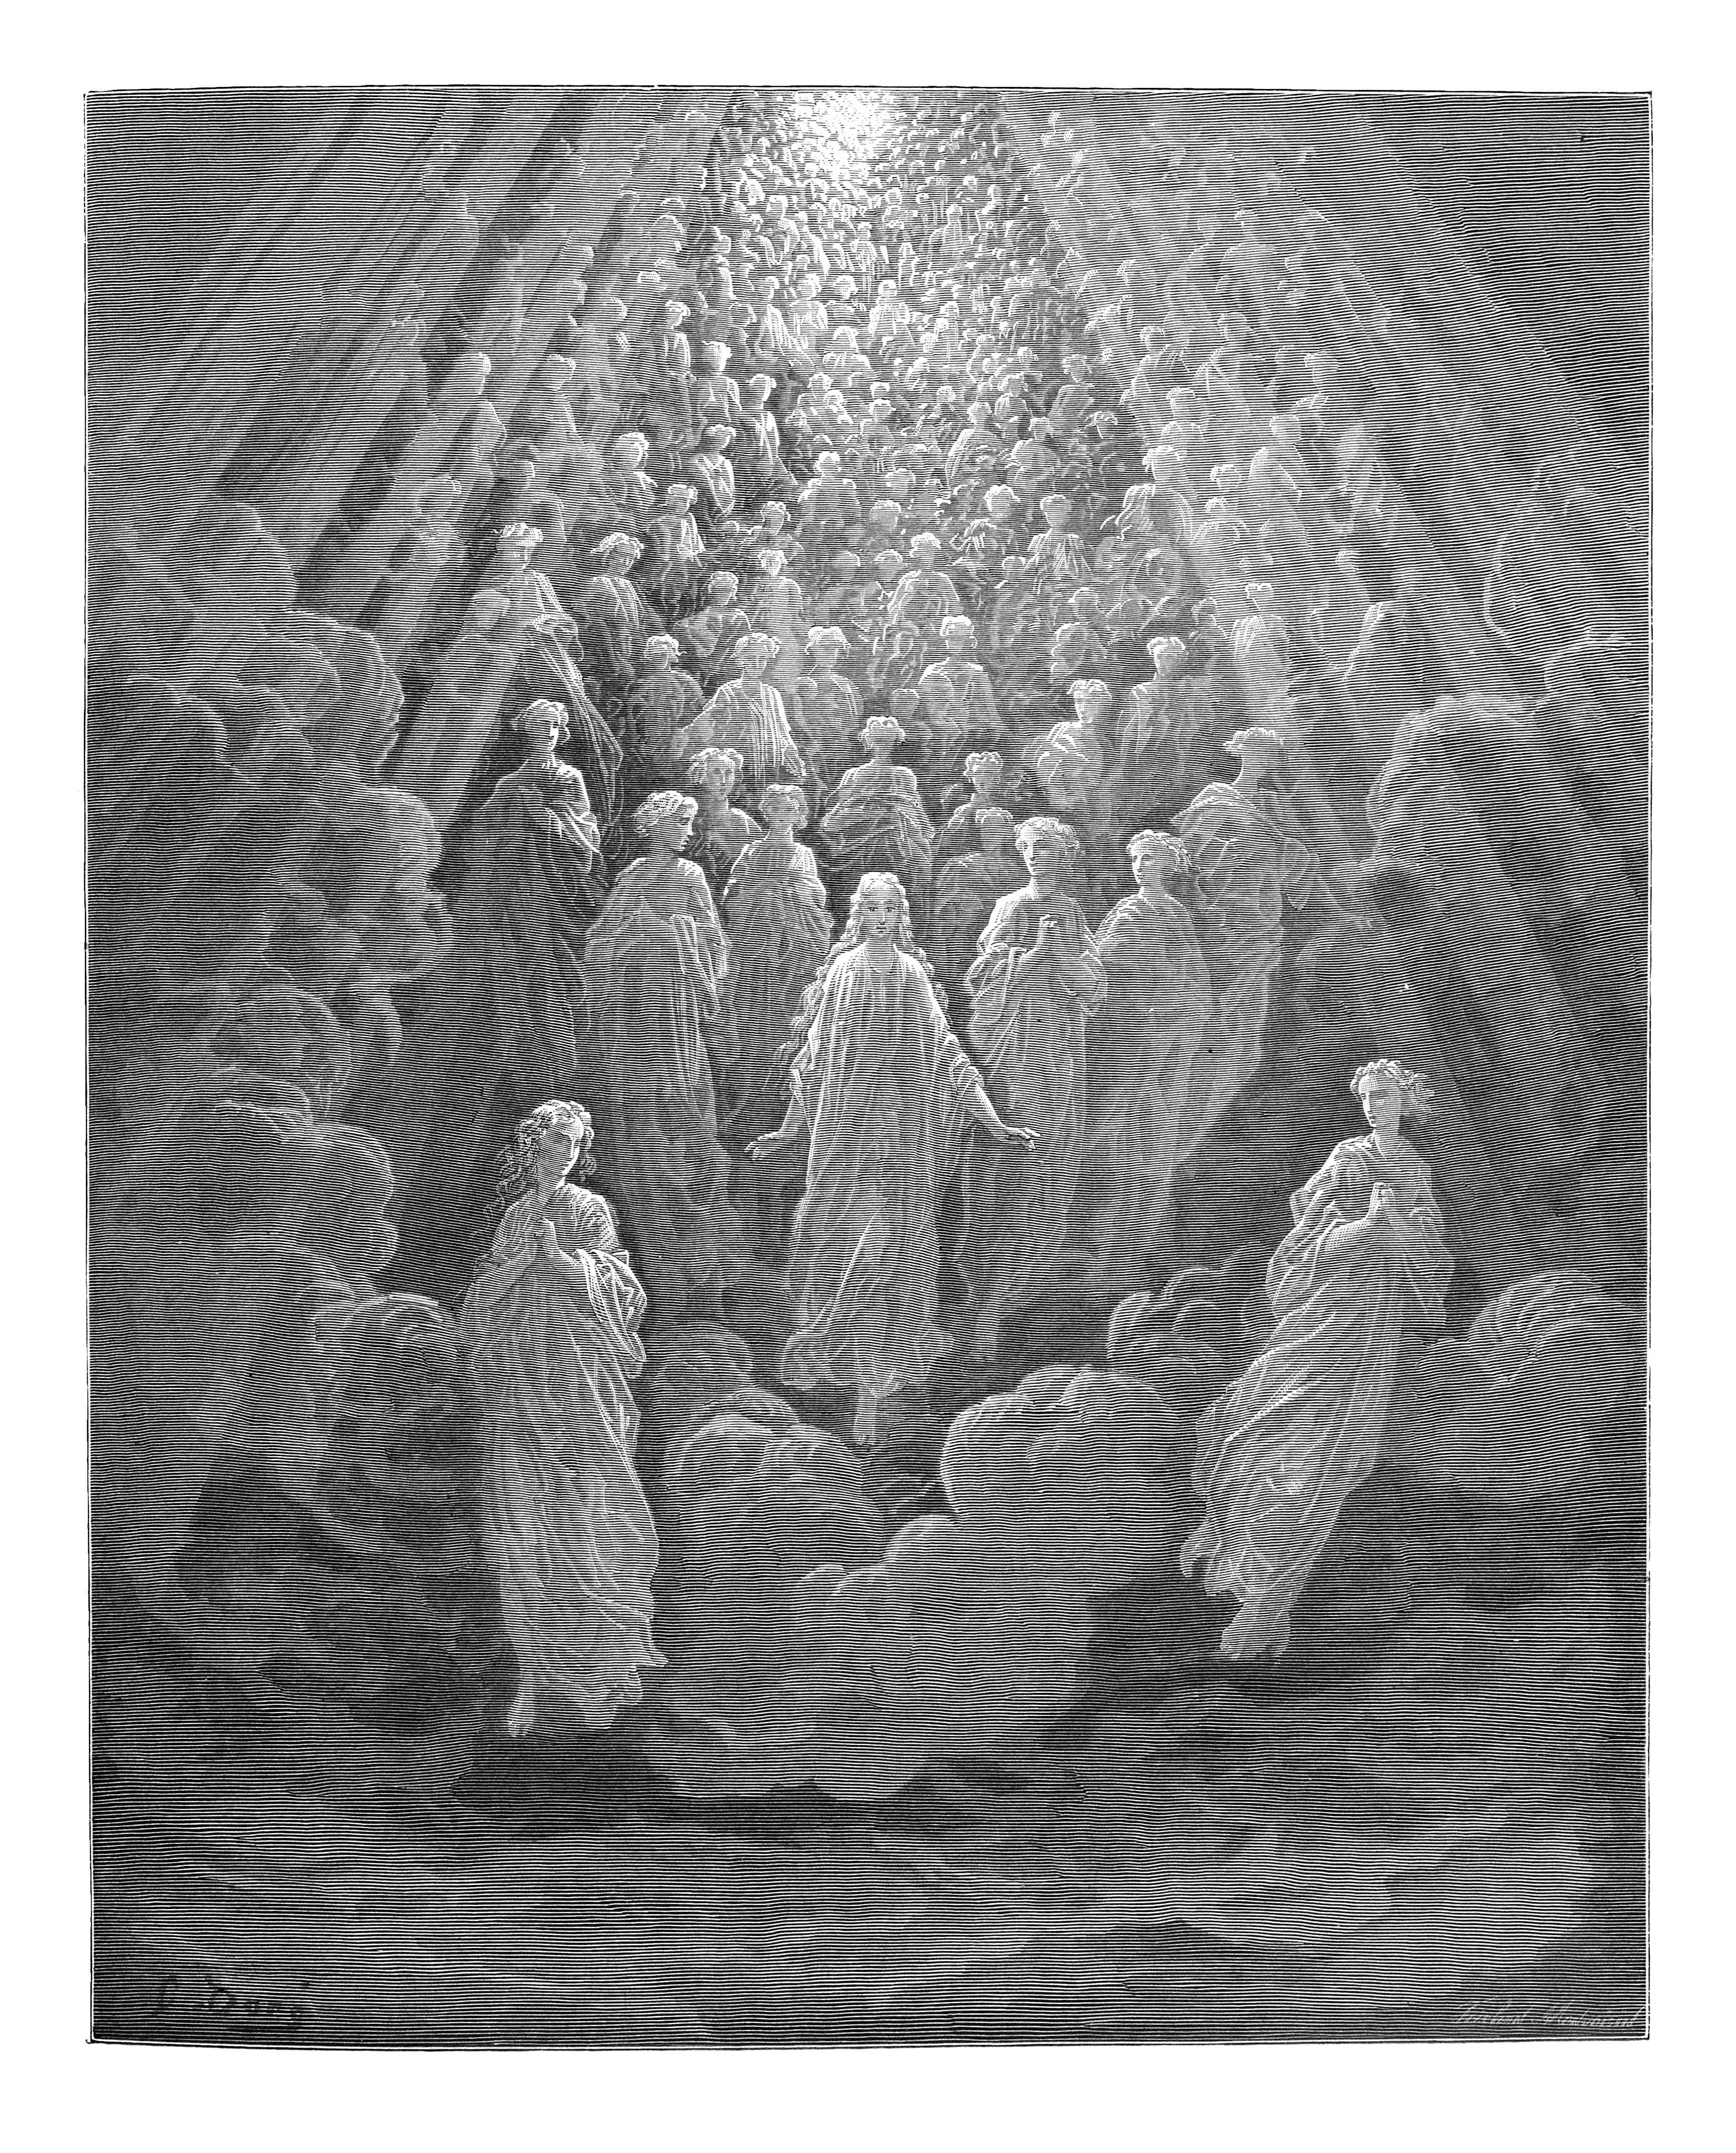
\includegraphics[height=\figsize]{illustrations/book_3/V03, c05.jpg}
\end{figure}

\begin{center}
\begin{minipage}{0.8\linewidth}
\textit{\\
"s\`{\i} vid’io ben più di mille splendori\\trarsi ver’ noi, e in ciascun s’ud\`{\i}a:"} \\
—V03, c05 \\~\\
\textit{"..so drew\\Full more than thousand splendours towards us, …"} \\
—B03, c05
\end{minipage}
\end{center}

\newpage

\section{Canto 08}

\begin{figure}[ht]
\centering
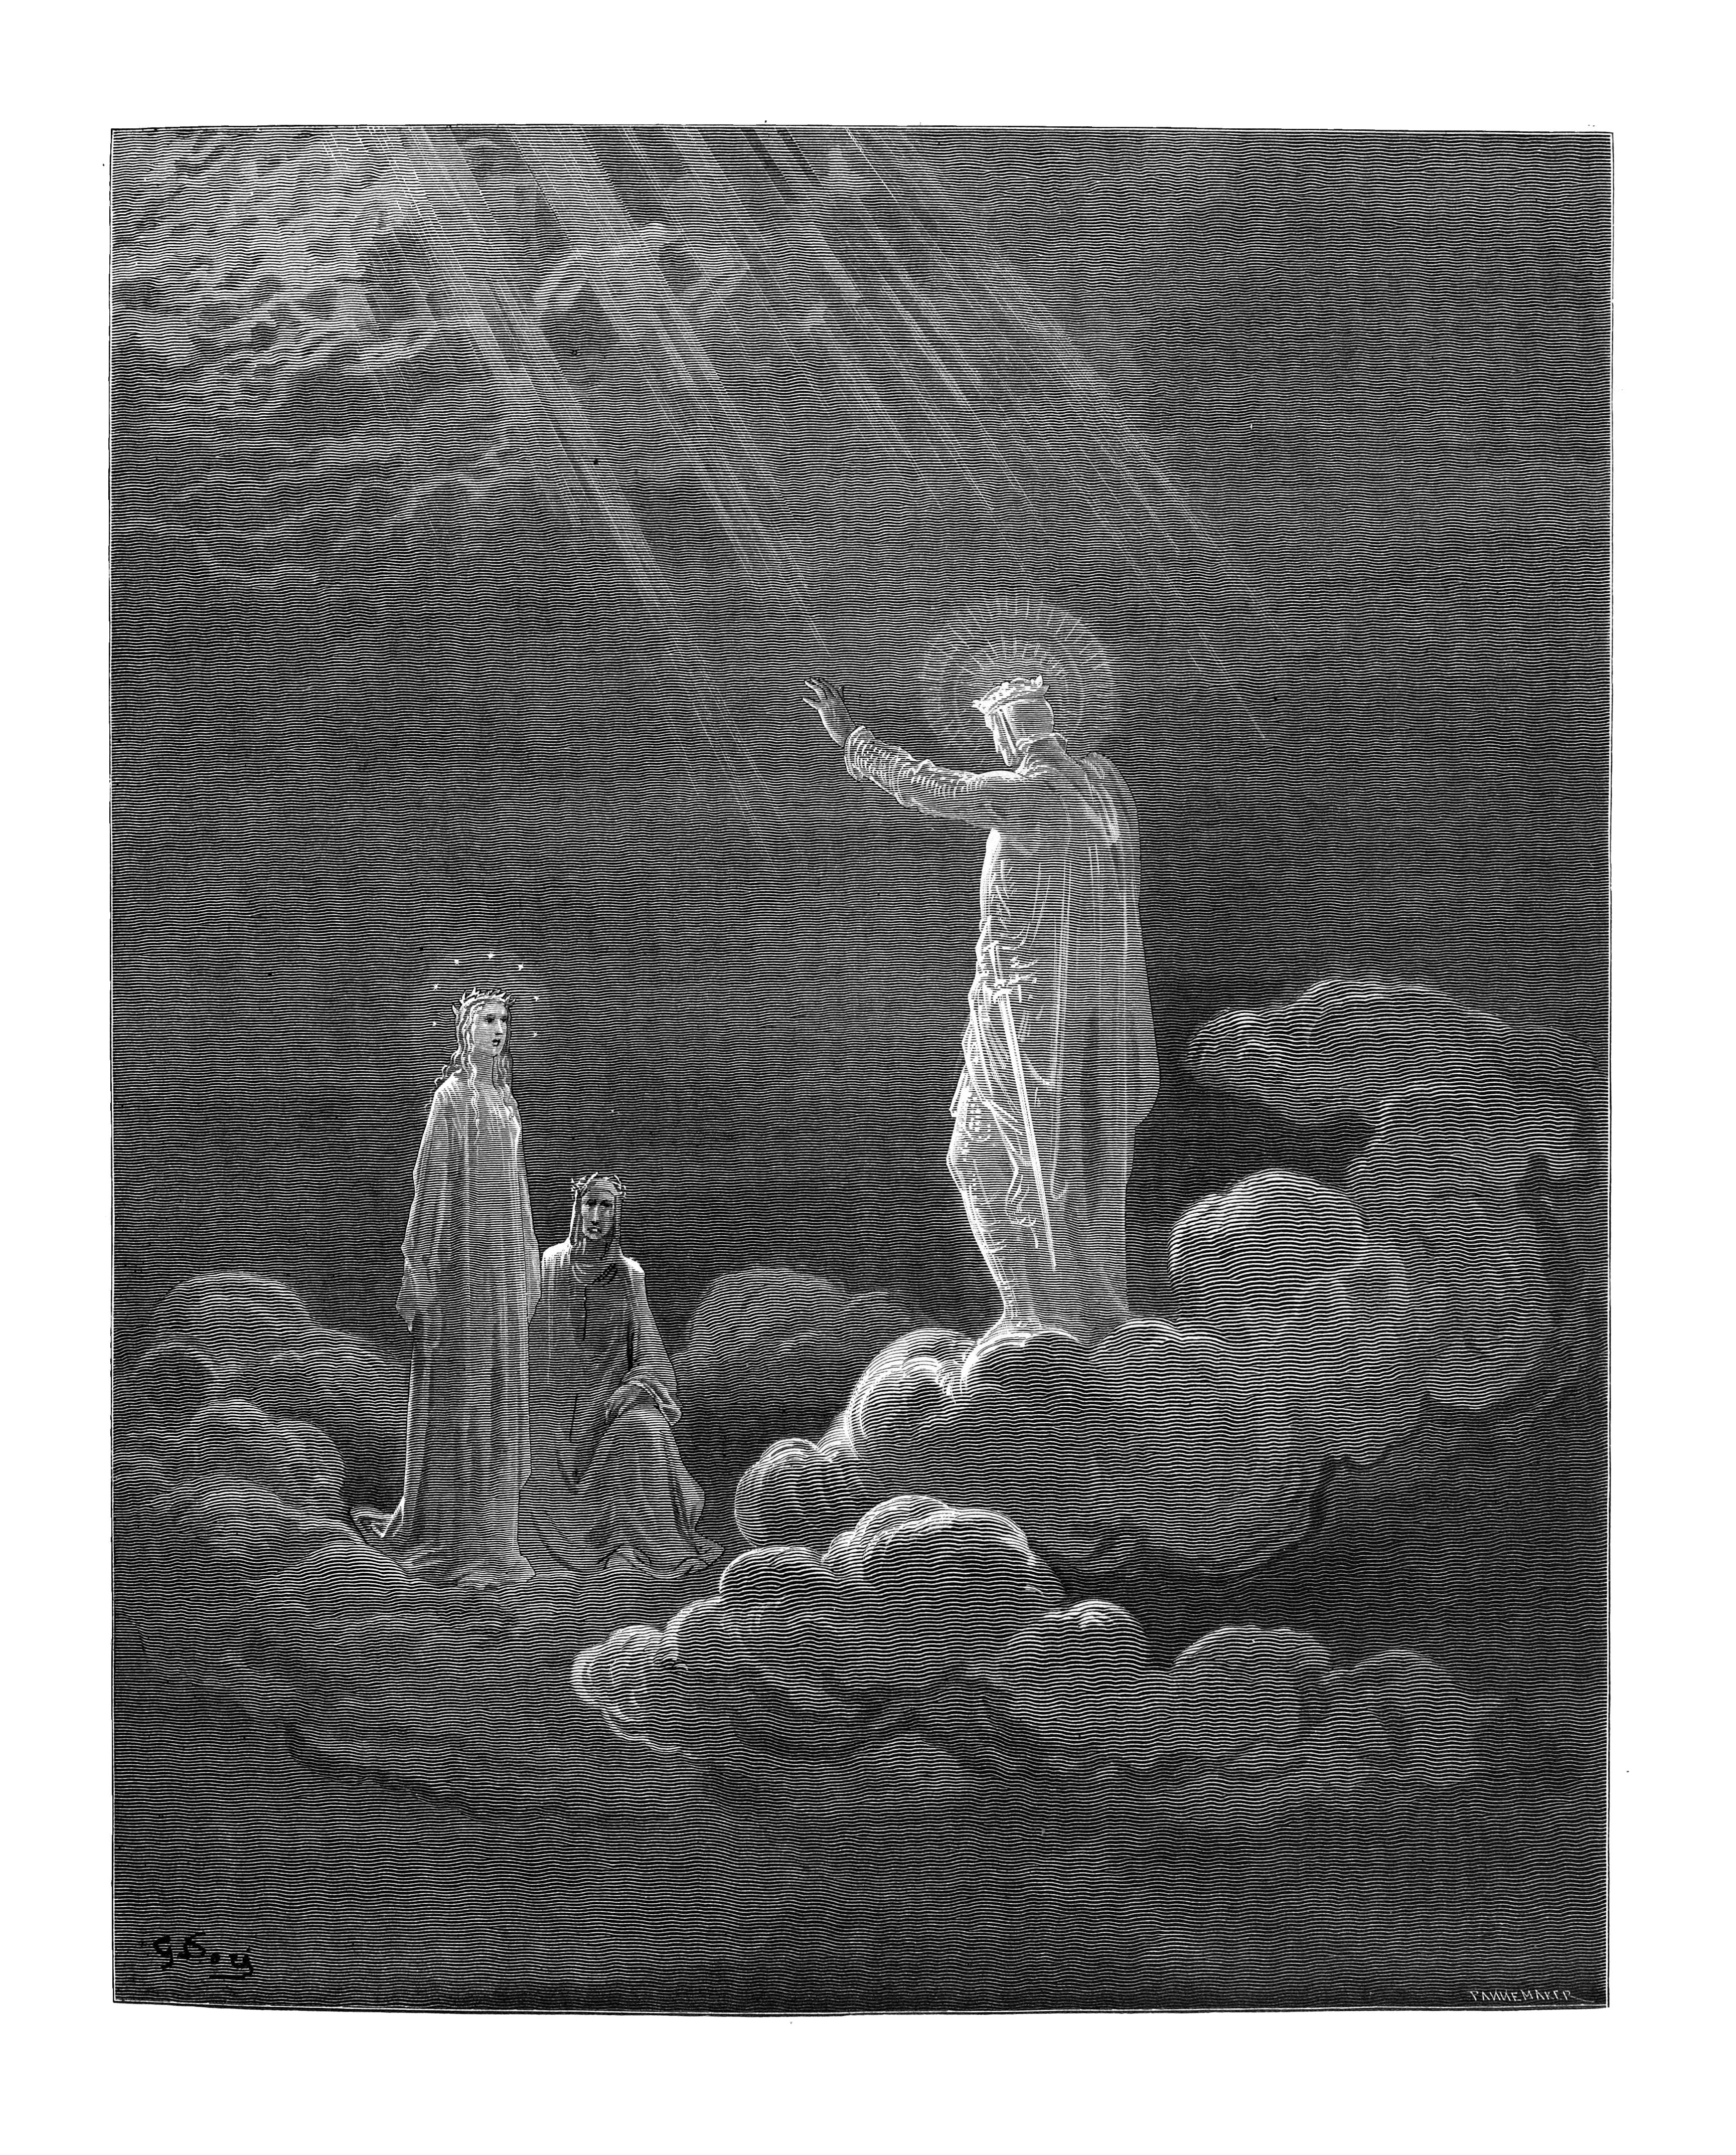
\includegraphics[height=\figsize]{illustrations/book_3/V03, c08.jpg}
\end{figure}

\begin{center}
\begin{minipage}{0.8\linewidth}
\textit{\\
"… «Il mondo m’ebbe\\giù poco tempo; e se più fosse stato,\\molto sarà di mal, che non sarebbe."} \\
—V03, c08 \\~\\
\textit{"\textquotesingle A short date below\\The world possess'd me. Had the time been more,\\Much evil, that will come, had never chanc'd. …"} \\
—B03, c08
\end{minipage}
\end{center}

\newpage

\section{Canto 12}

\begin{figure}[ht]
\centering
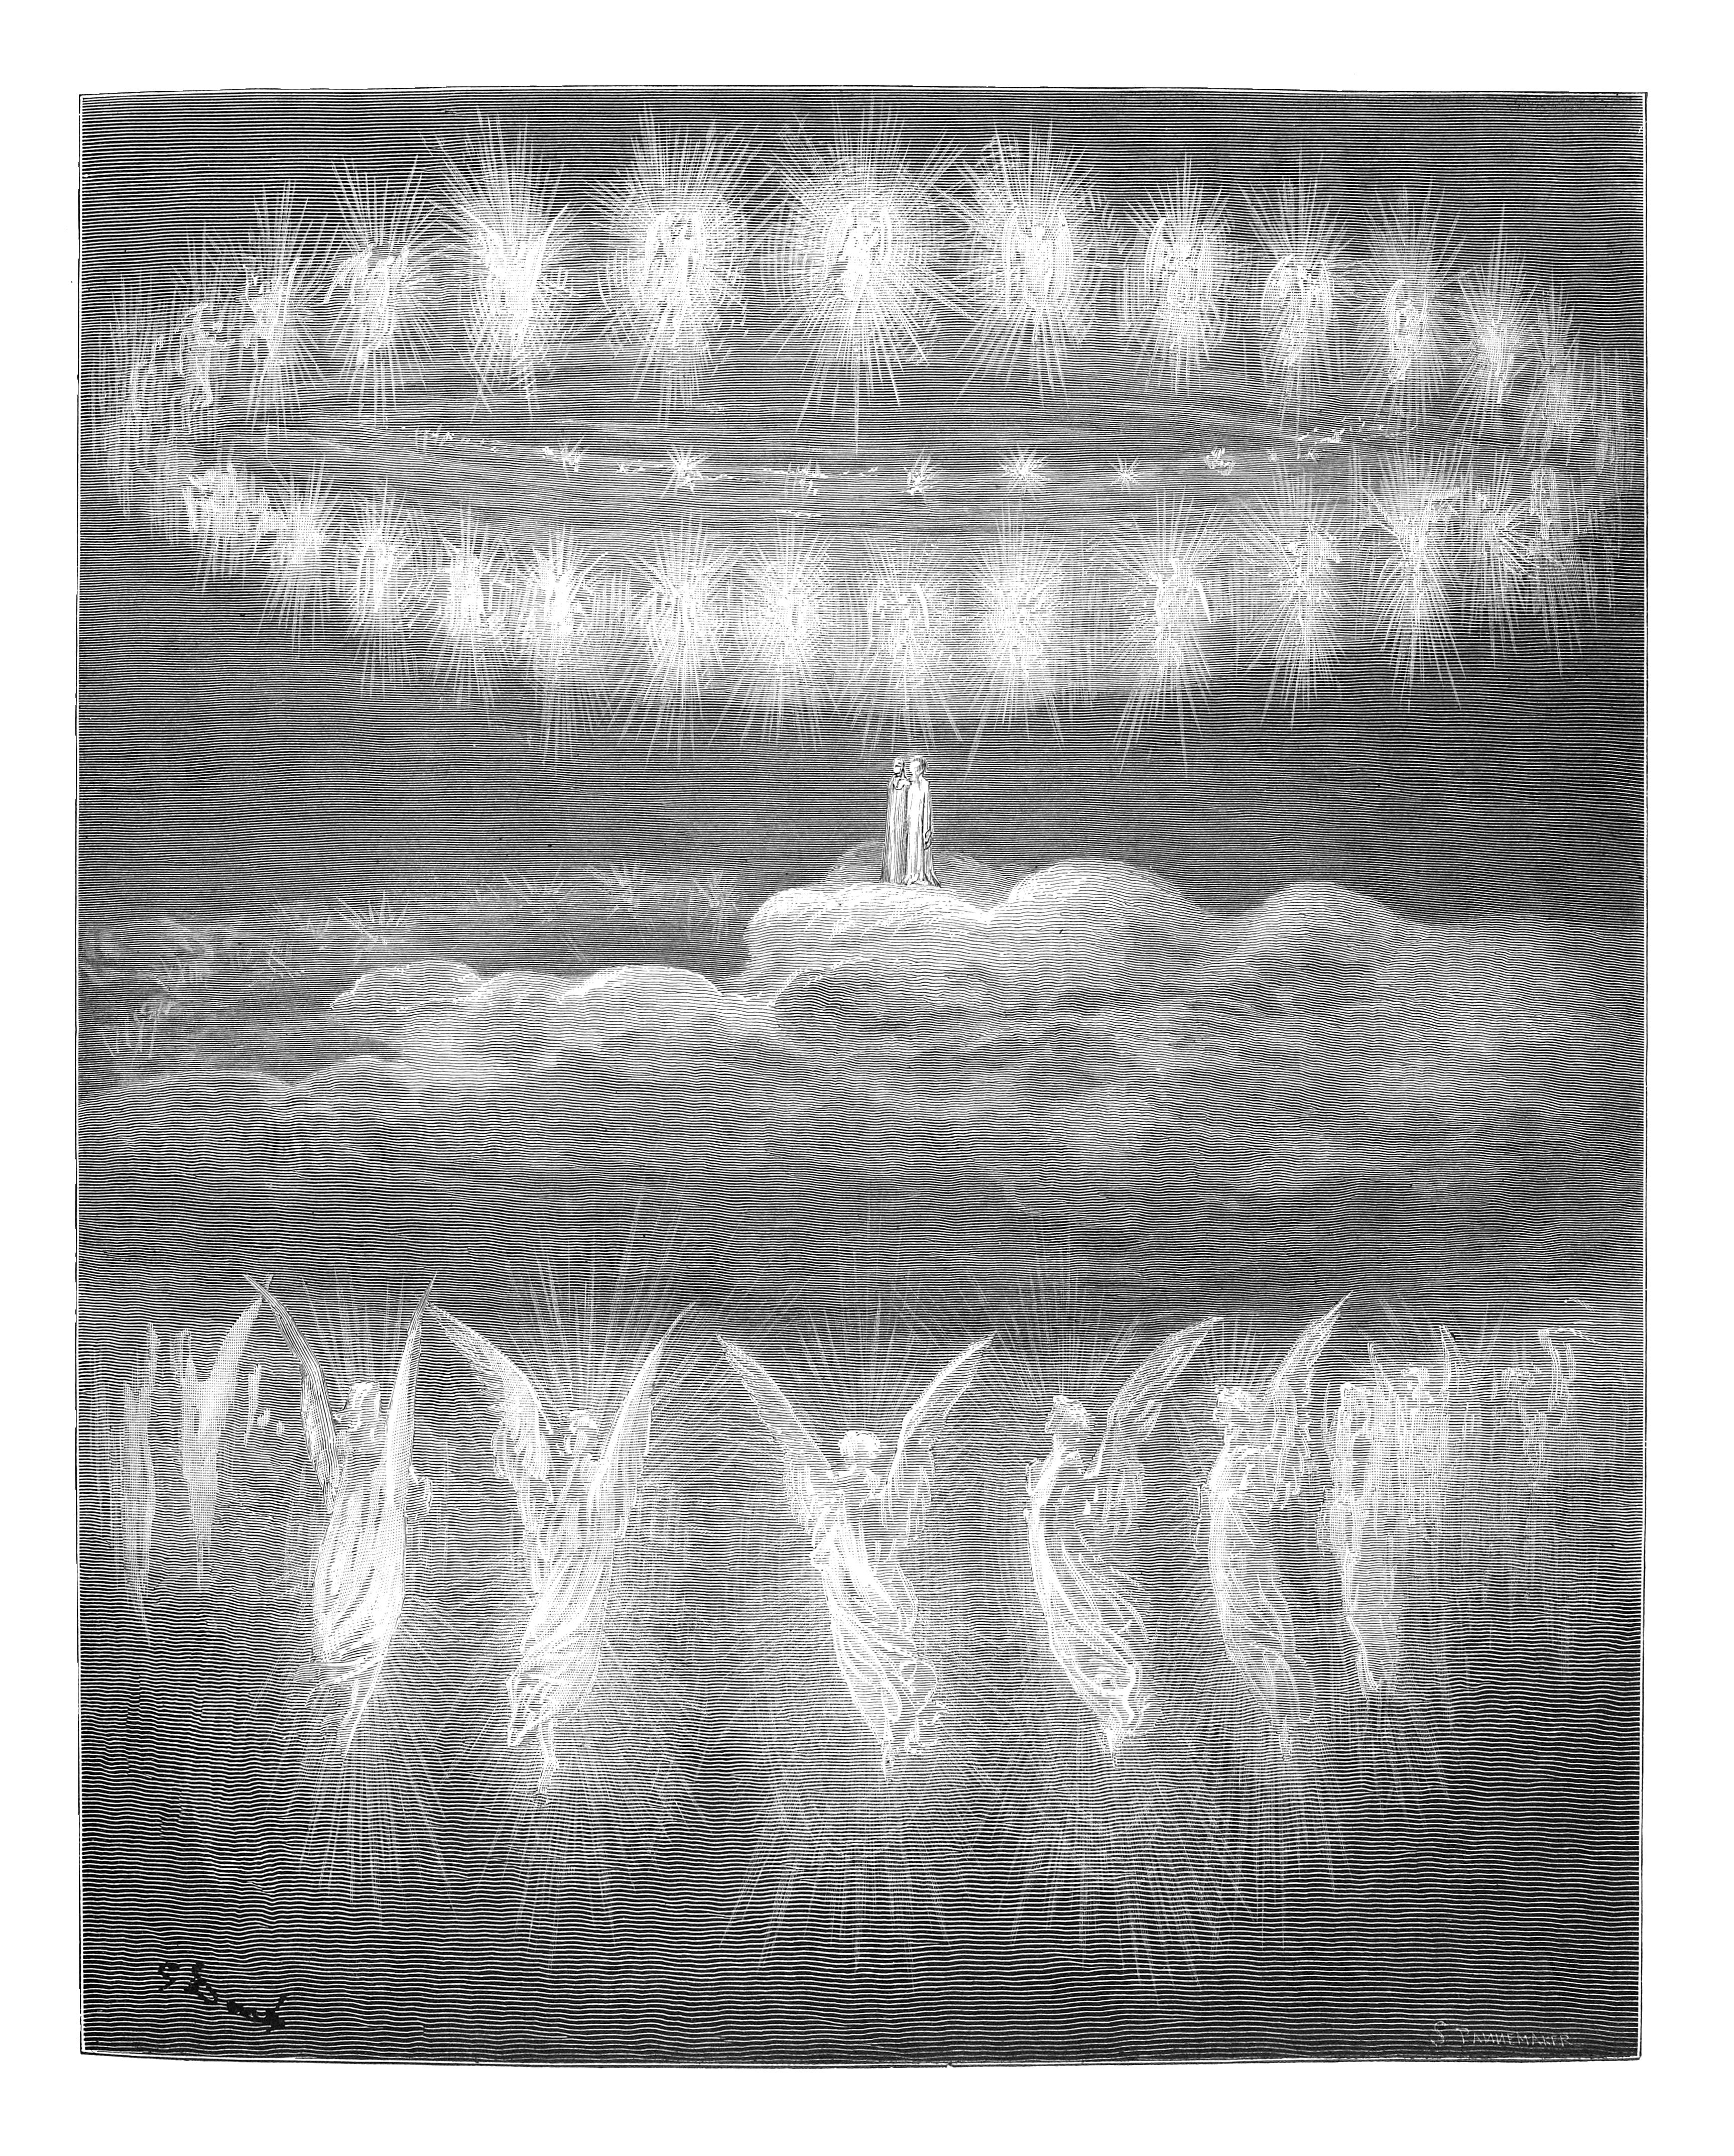
\includegraphics[height=\figsize]{illustrations/book_3/V03, c12.jpg}
\end{figure}

\begin{center}
\begin{minipage}{0.8\linewidth}
\textit{\\
"a rotar cominciò la santa mola;\\e nel suo giro tutta non si volse\\prima ch’un’altra di cerchio la chiuse,"} \\
—V03, c12 \\~\\
\textit{"...straight the holy mill\\Began to wheel, nor yet had once revolv'd,\\Or ere another, circling, compass'd it,"} \\
—B03, c12
\end{minipage}
\end{center}

\newpage

\section{Canto 14(1)}

\begin{figure}[ht]
\centering
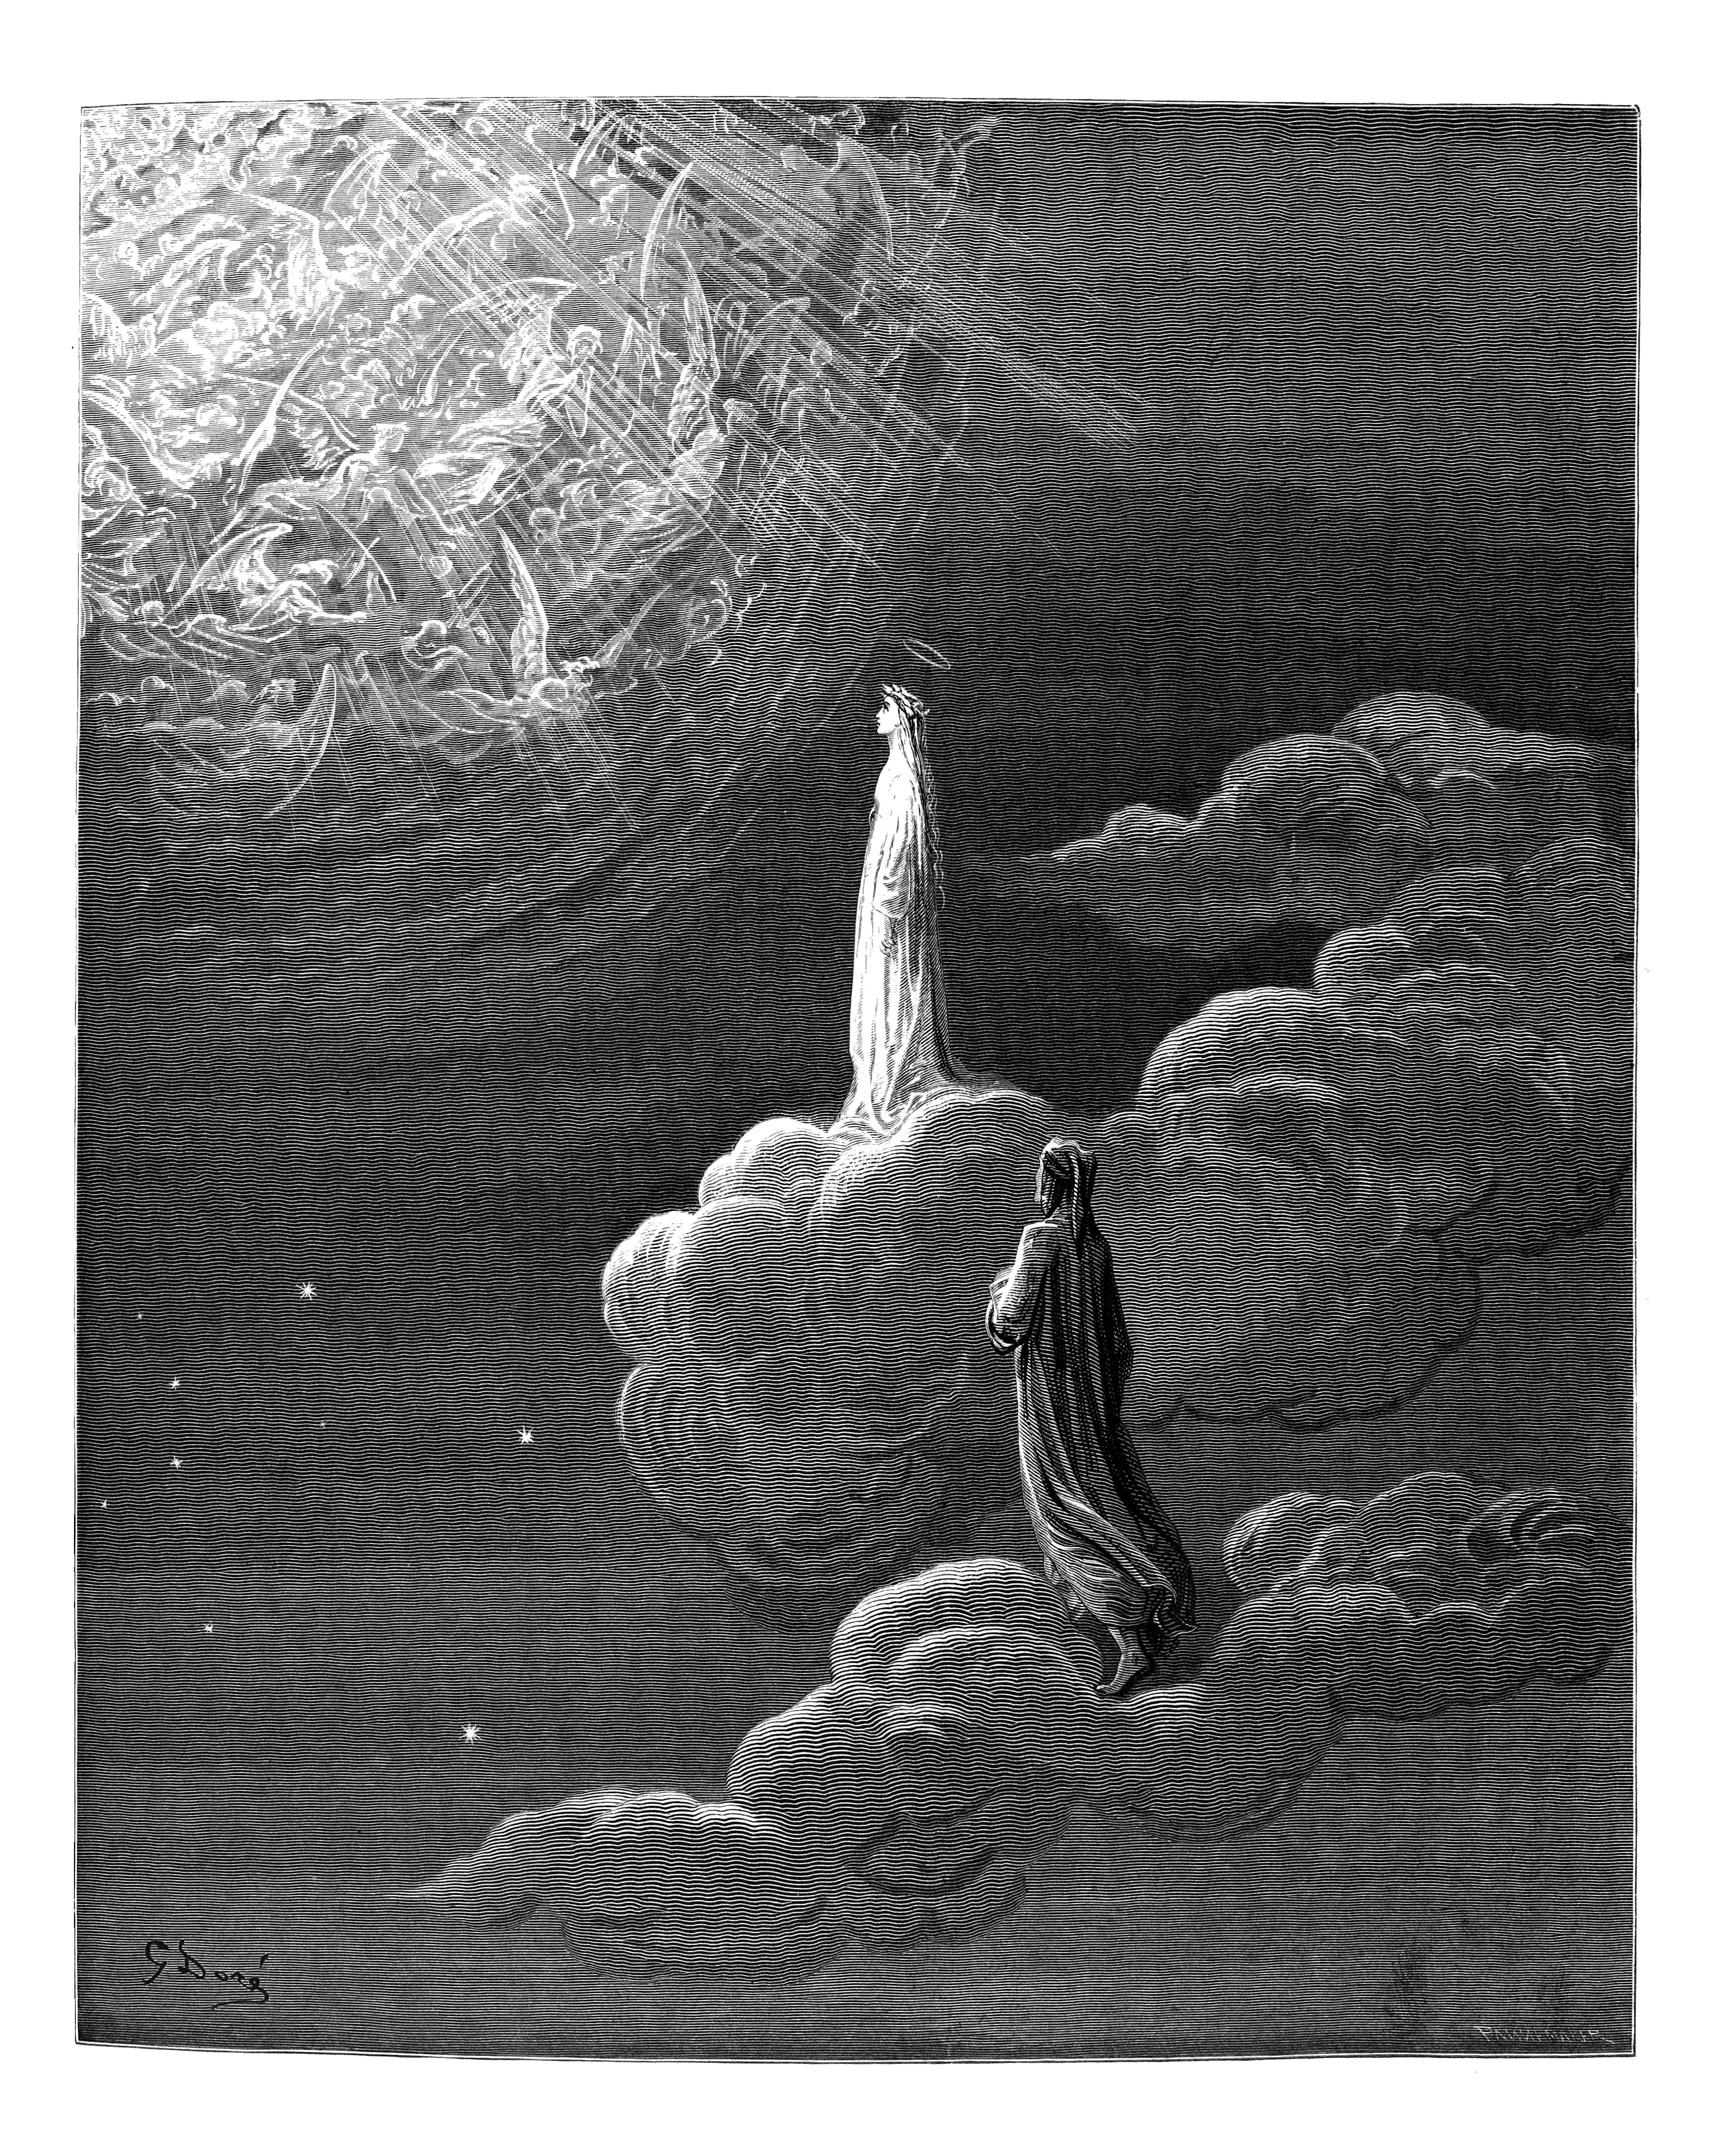
\includegraphics[height=\figsize]{illustrations/book_3/V03, c14(1).jpg}
\end{figure}

\begin{center}
\begin{minipage}{0.8\linewidth}
\textit{\\
"...con tanto lucore e tanto robbi\\m’apparvero splendor dentro a due raggi,"} \\
—V03, c14(1) \\~\\
\textit{"...With such mighty sheen\\And mantling crimson, in two listed rays\\The splendours shot before me,"} \\
—B03, c14(1)
\end{minipage}
\end{center}

\newpage

\section{Canto 14(2)}

\begin{figure}[ht]
\centering
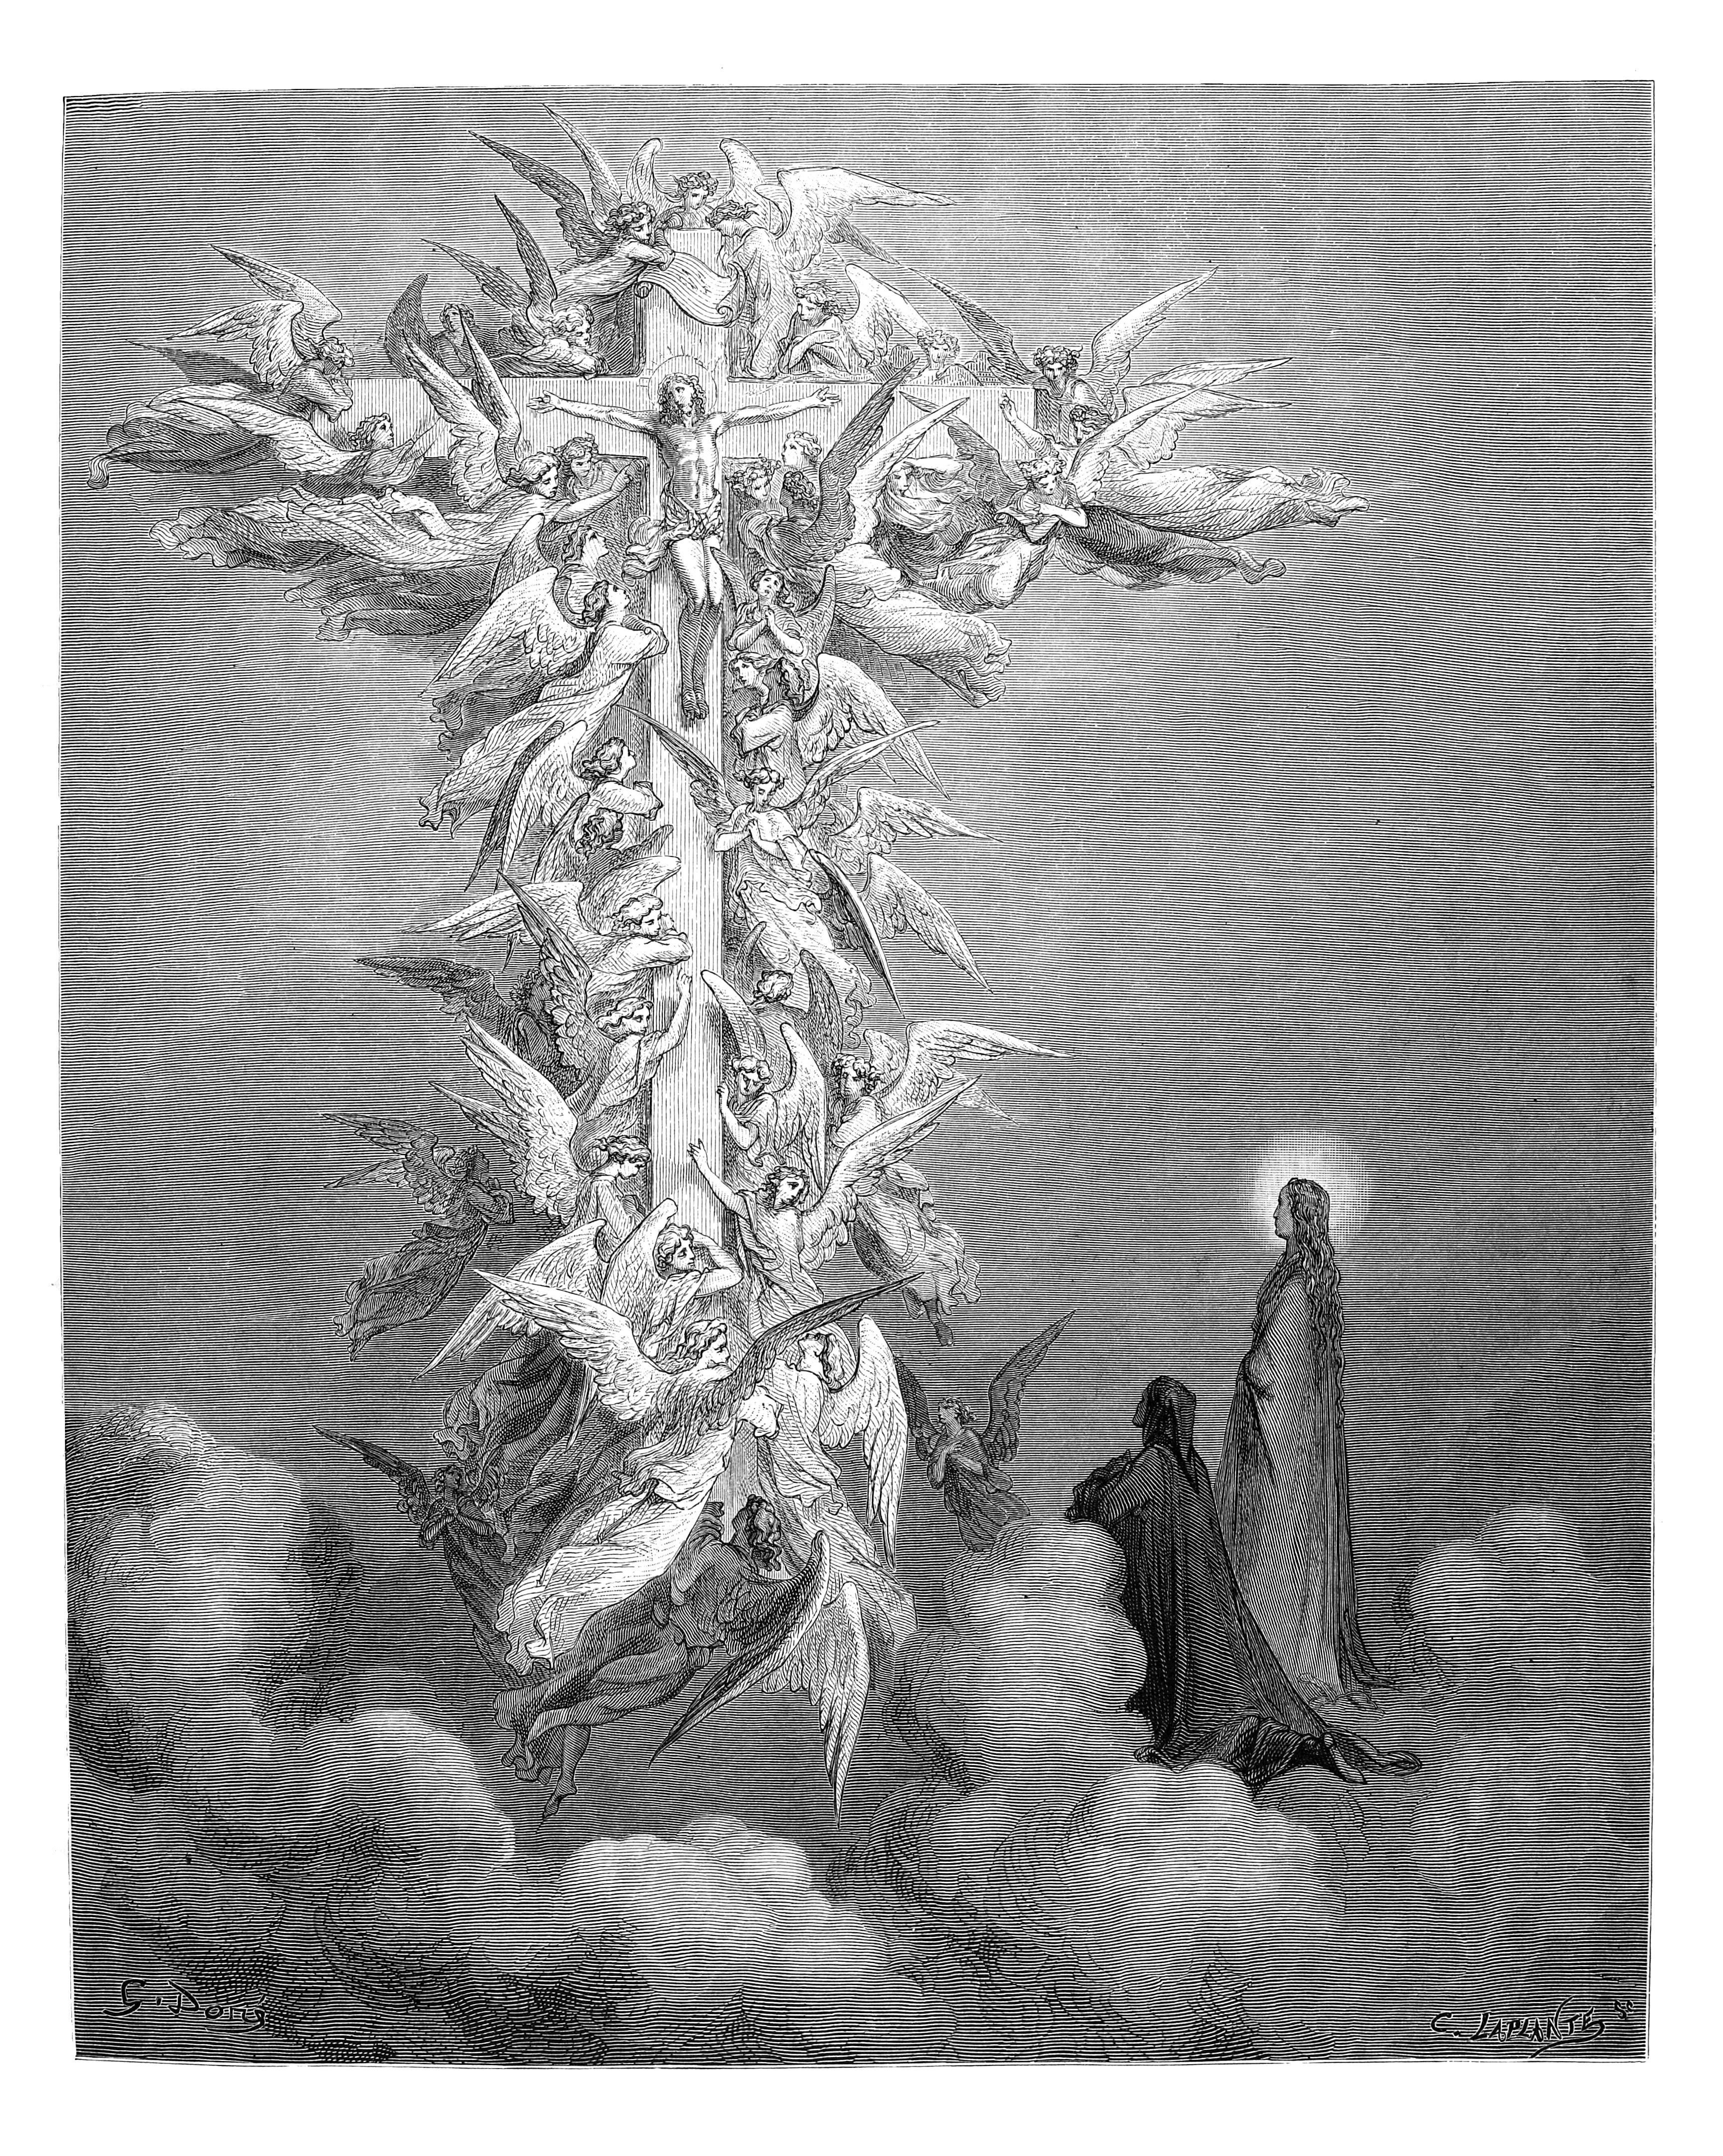
\includegraphics[height=\figsize]{illustrations/book_3/V03, c14(2).jpg}
\end{figure}

\begin{center}
\begin{minipage}{0.8\linewidth}
\textit{\\
"...quella croce lampeggiava Cristo,"} \\
—V03, c14(2) \\~\\
\textit{"…Christ\\Beam'd on that cross; ..."} \\
—B03, c14(2)
\end{minipage}
\end{center}

\newpage

\section{Canto 16}

\begin{figure}[ht]
\centering
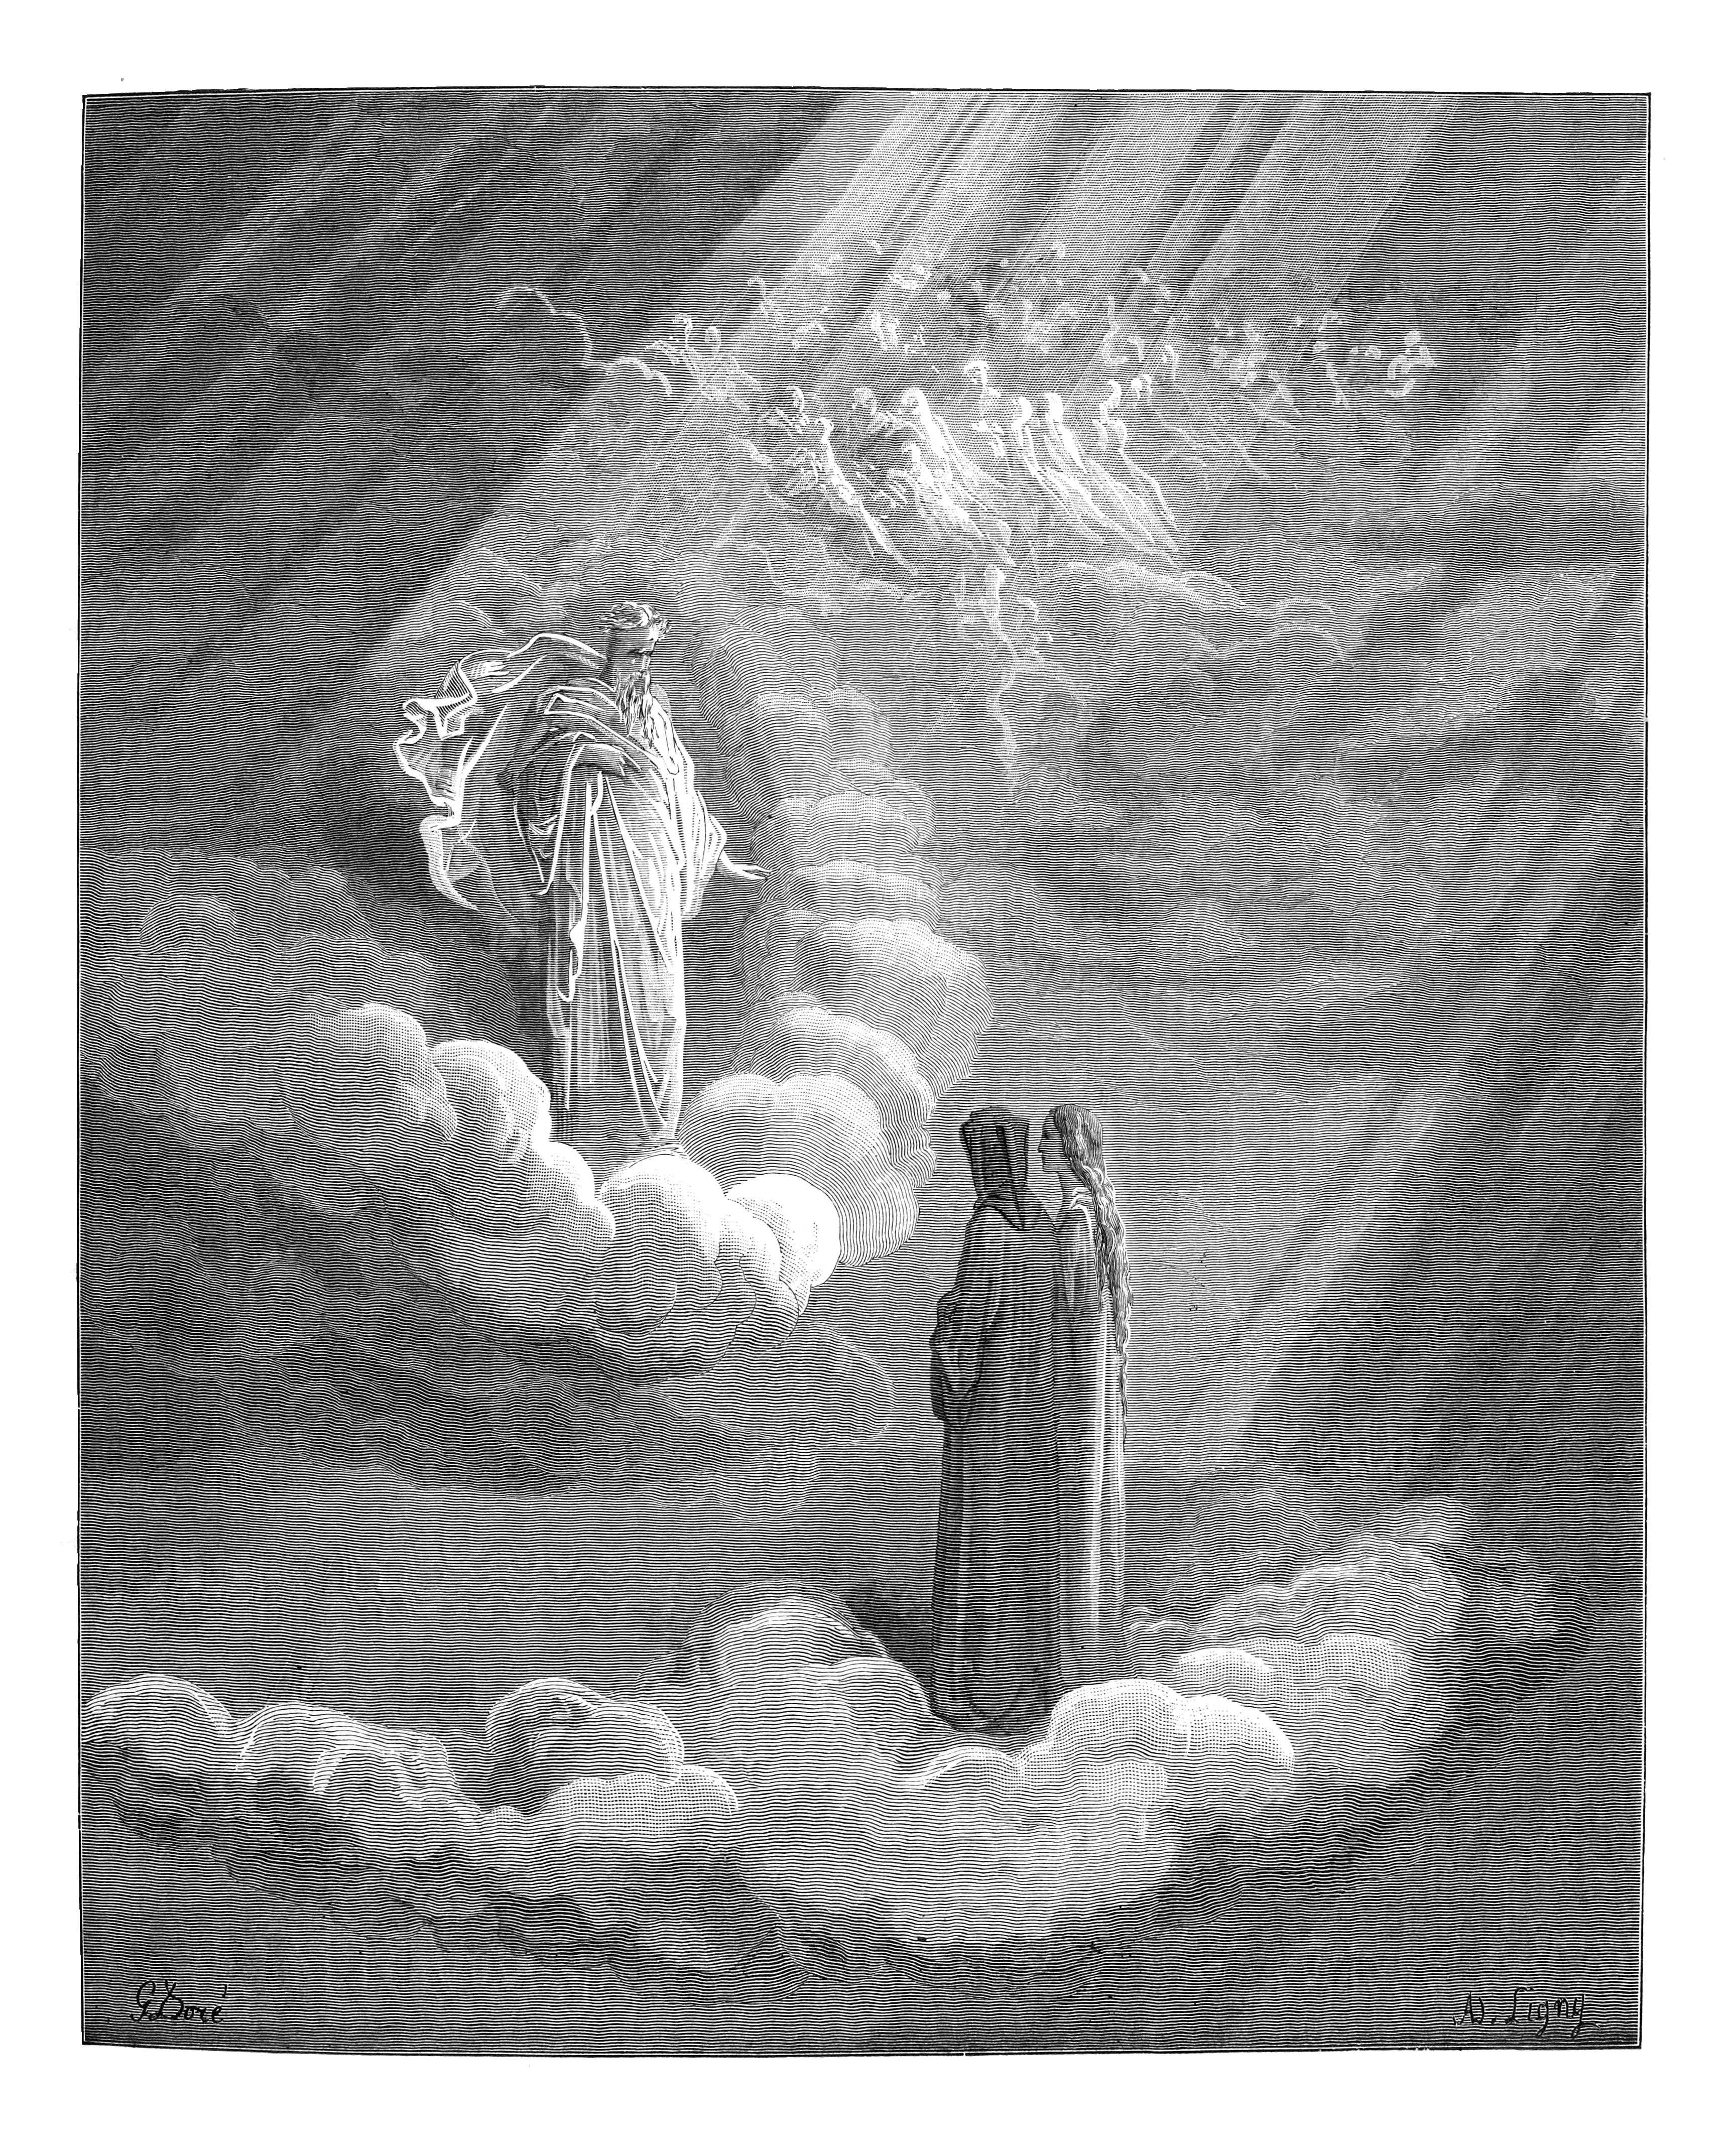
\includegraphics[height=\figsize]{illustrations/book_3/V03, c16.jpg}
\end{figure}

\begin{center}
\begin{minipage}{0.8\linewidth}
\textit{\\
"...conveniesi a quella pietra scema\\che guarda ’l ponte, che Fiorenza fesse\\vittima ne la sua pace postrema."} \\
—V03, c16 \\~\\
\textit{"...so was doom'd:\\On that maim'd stone set up to guard the bridge,\\At thy last peace, the victim, Florence! fell."} \\
—B03, c16
\end{minipage}
\end{center}

\newpage

\section{Canto 18(1)}

\begin{figure}[ht]
\centering
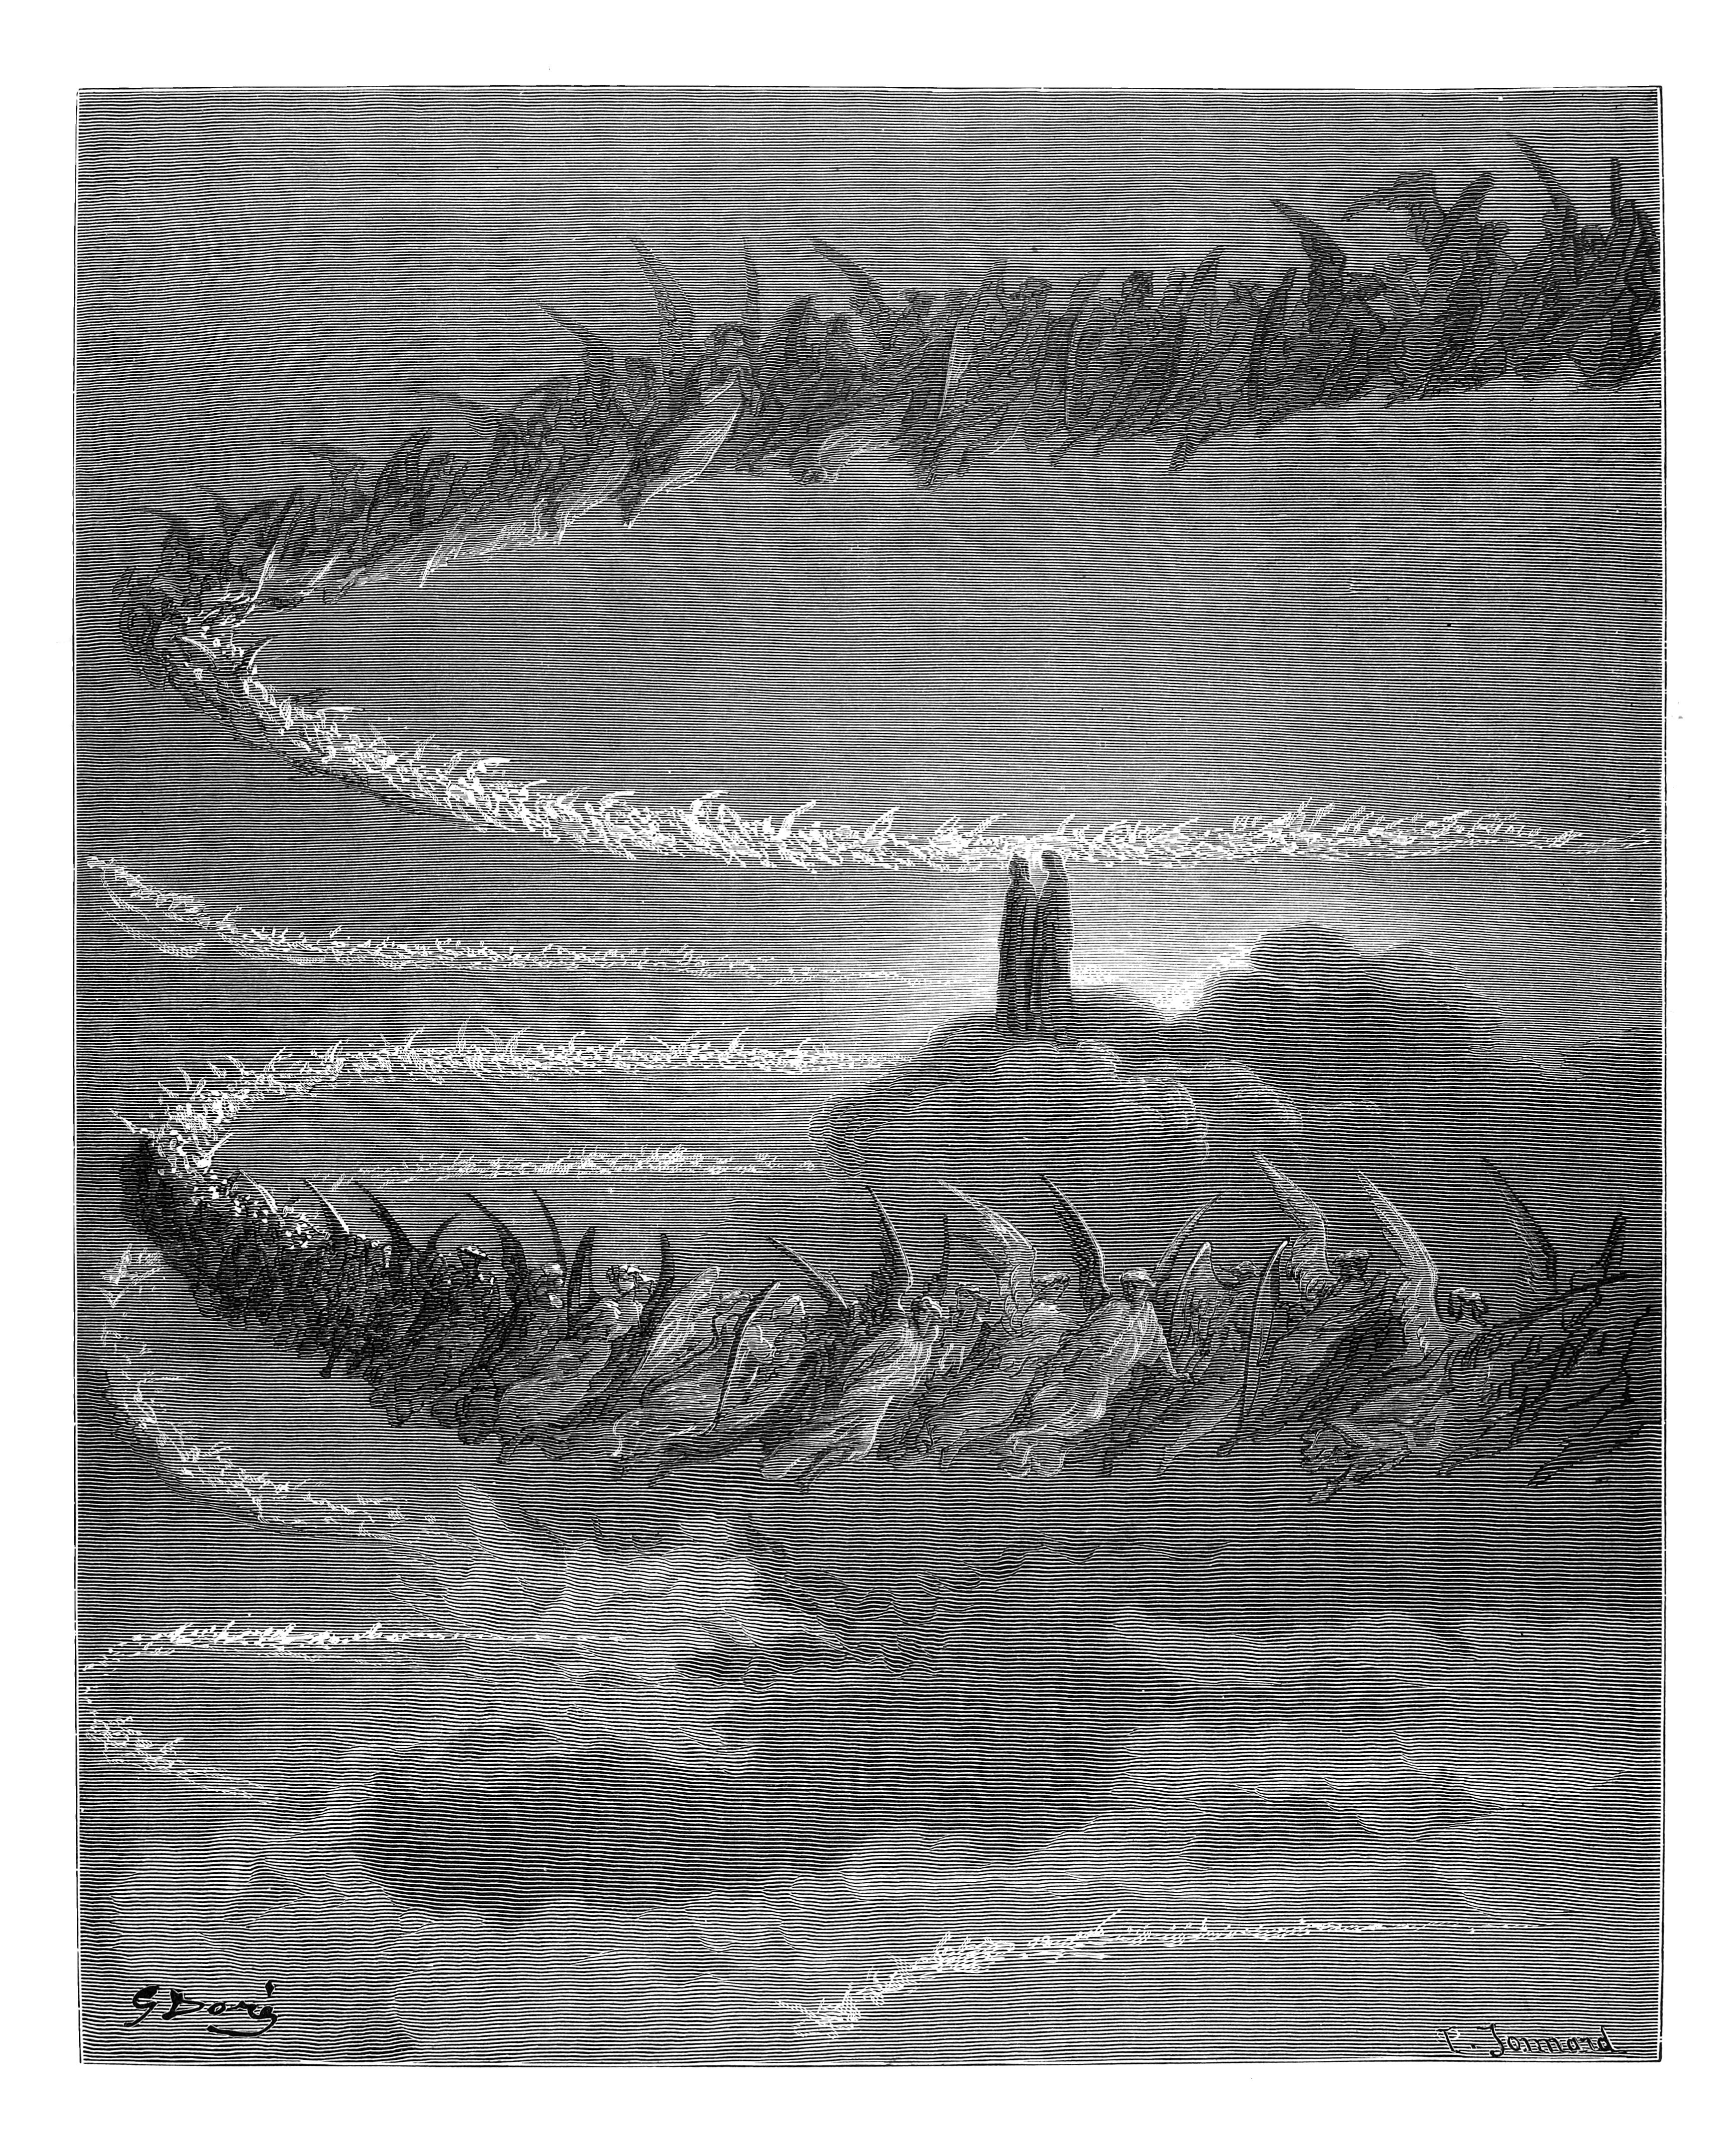
\includegraphics[height=\figsize]{illustrations/book_3/V03, c18(1).jpg}
\end{figure}

\begin{center}
\begin{minipage}{0.8\linewidth}
\textit{\\
"resurger parver quindi più di mille\\luci e salir, …"} \\
—V03, c18(1) \\~\\
\textit{"Thus more than thousand twinkling lustres hence\\Seem'd reascending, …"} \\
—B03, c18(1)
\end{minipage}
\end{center}

\newpage

\section{Canto 18(2)}

\begin{figure}[ht]
\centering
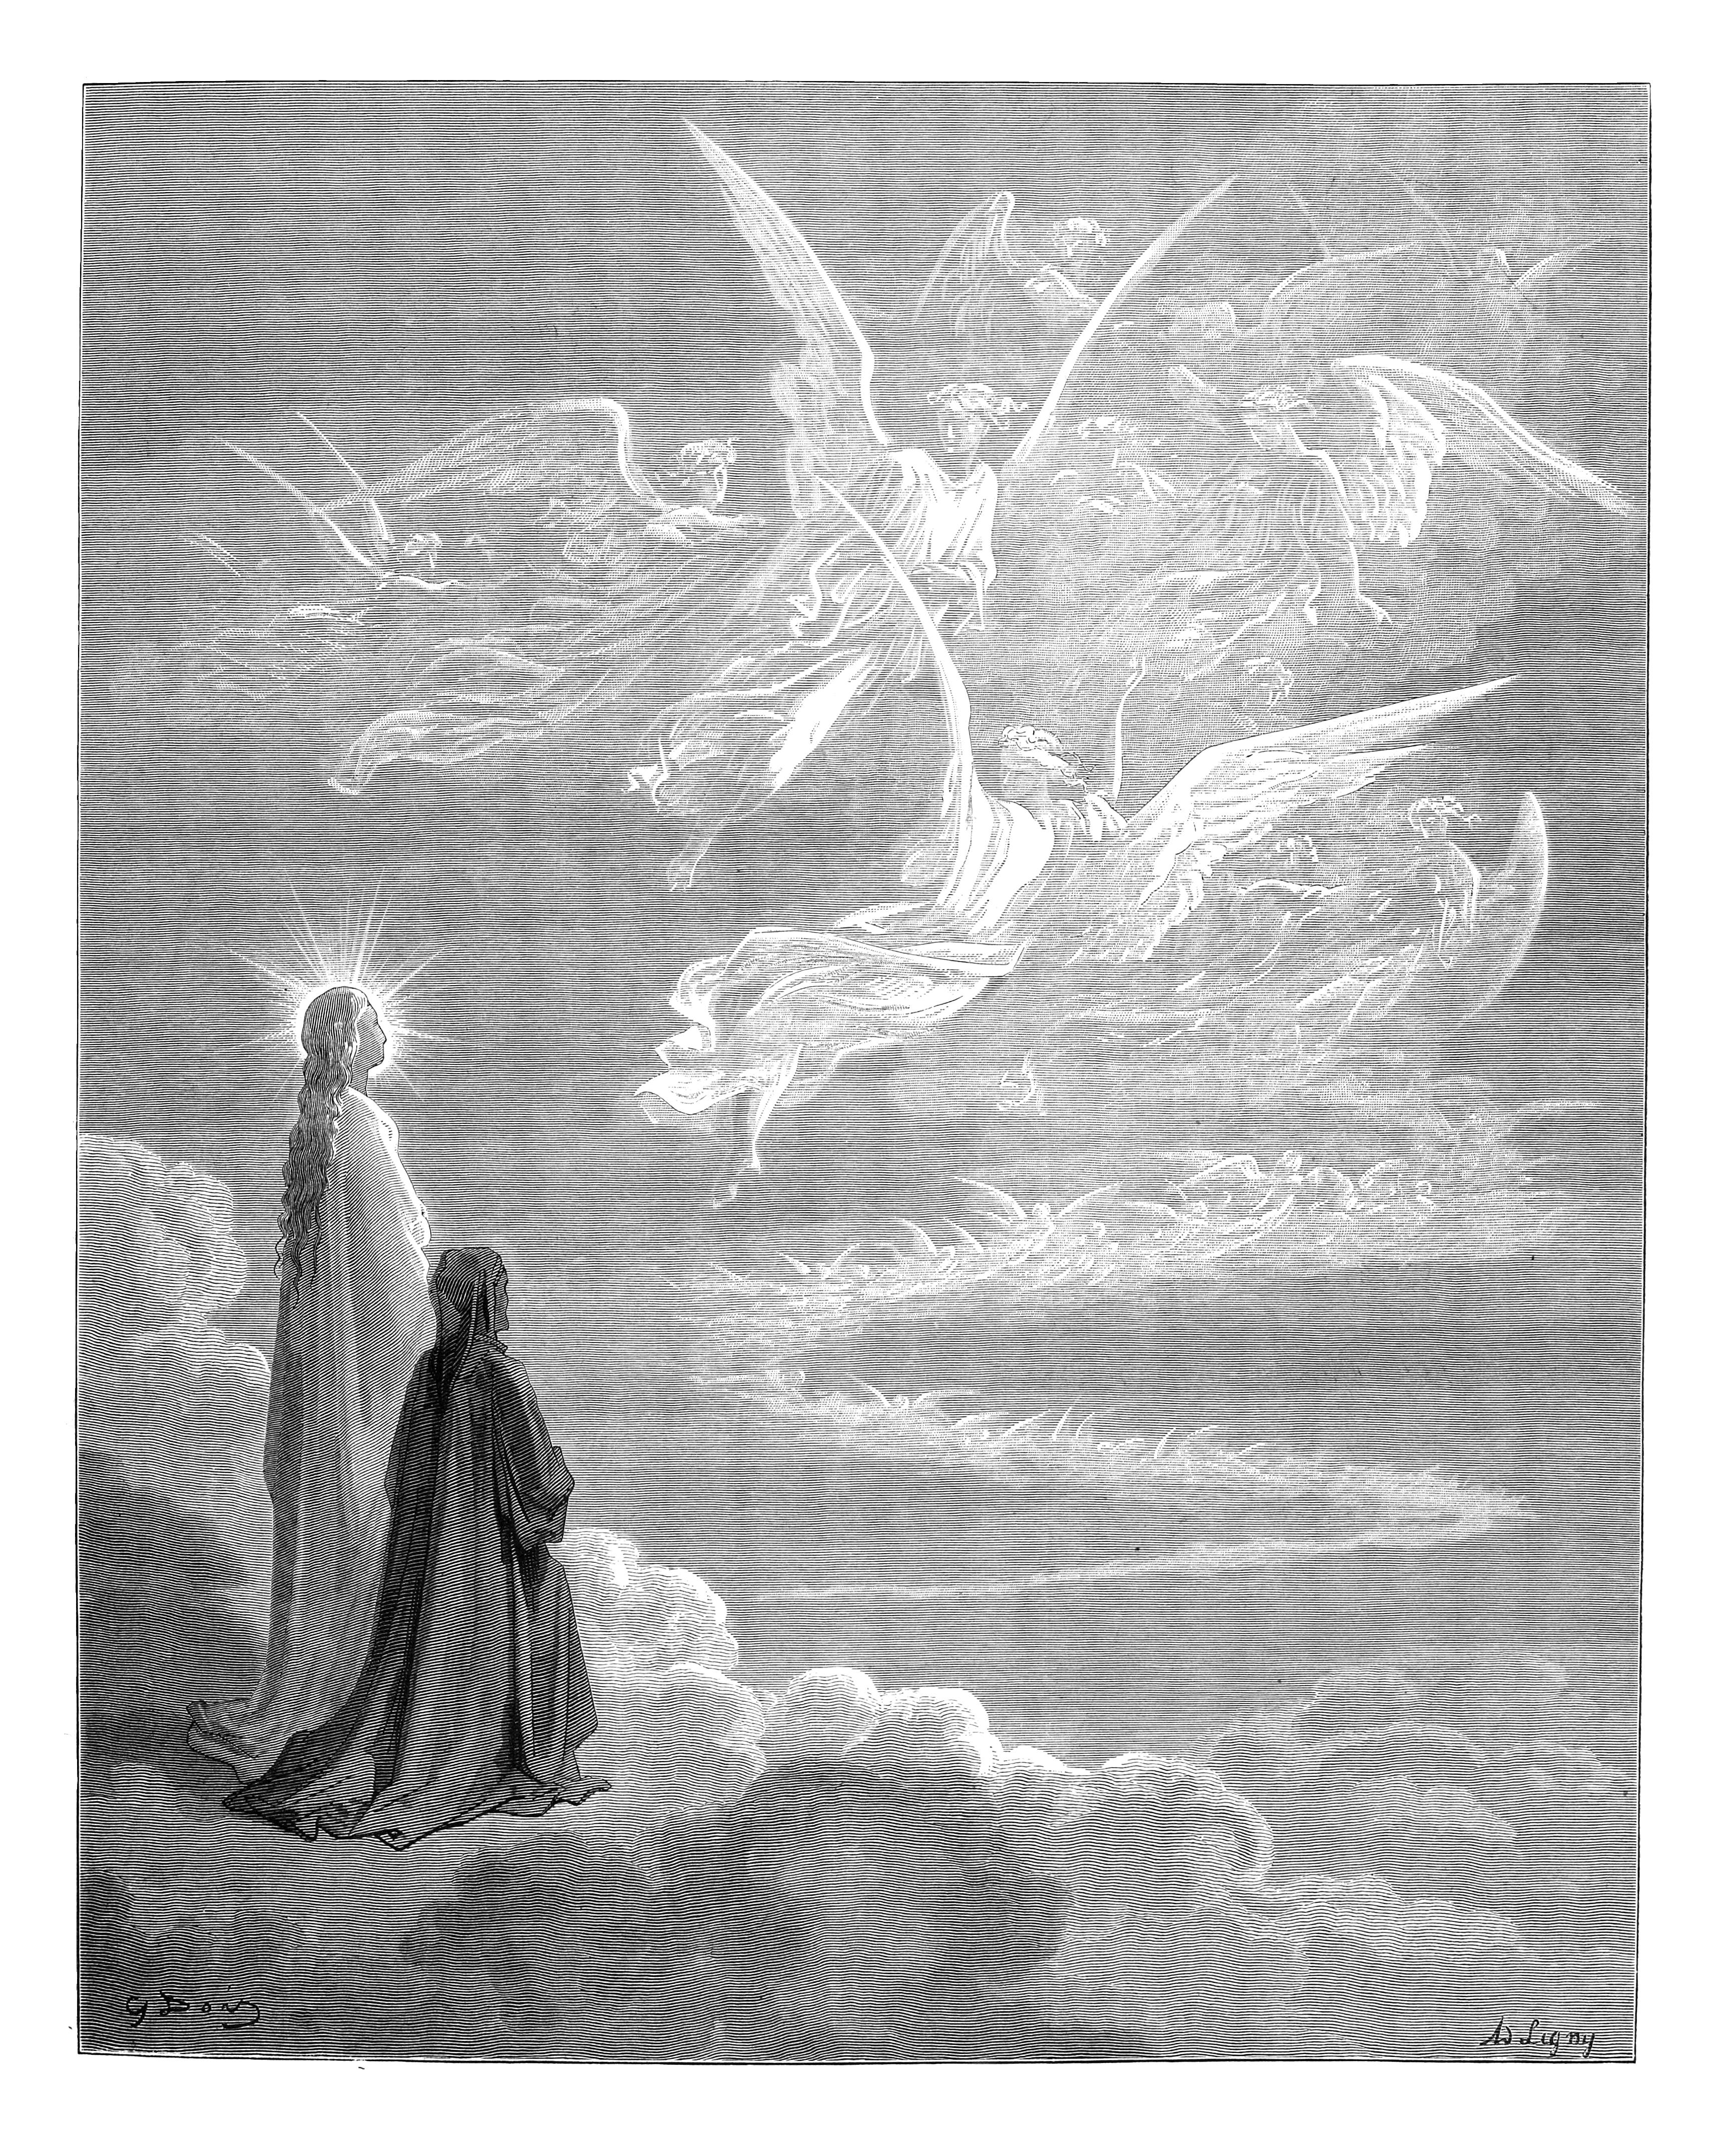
\includegraphics[height=\figsize]{illustrations/book_3/V03, c18(2).jpg}
\end{figure}

\begin{center}
\begin{minipage}{0.8\linewidth}
\textit{\\
"O milizia del ciel cu’ io contemplo,\\adora per color che sono in terra\\tutti sviati dietro al malo essemplo!"} \\
—V03, c18(2) \\~\\
\textit{"Ye host of heaven! whose glory I survey!\\O beg ye grace for those, that are on earth\\All after ill example gone astray."} \\
—B03, c18(2)
\end{minipage}
\end{center}

\newpage

\section{Canto 19}

\begin{figure}[ht]
\centering
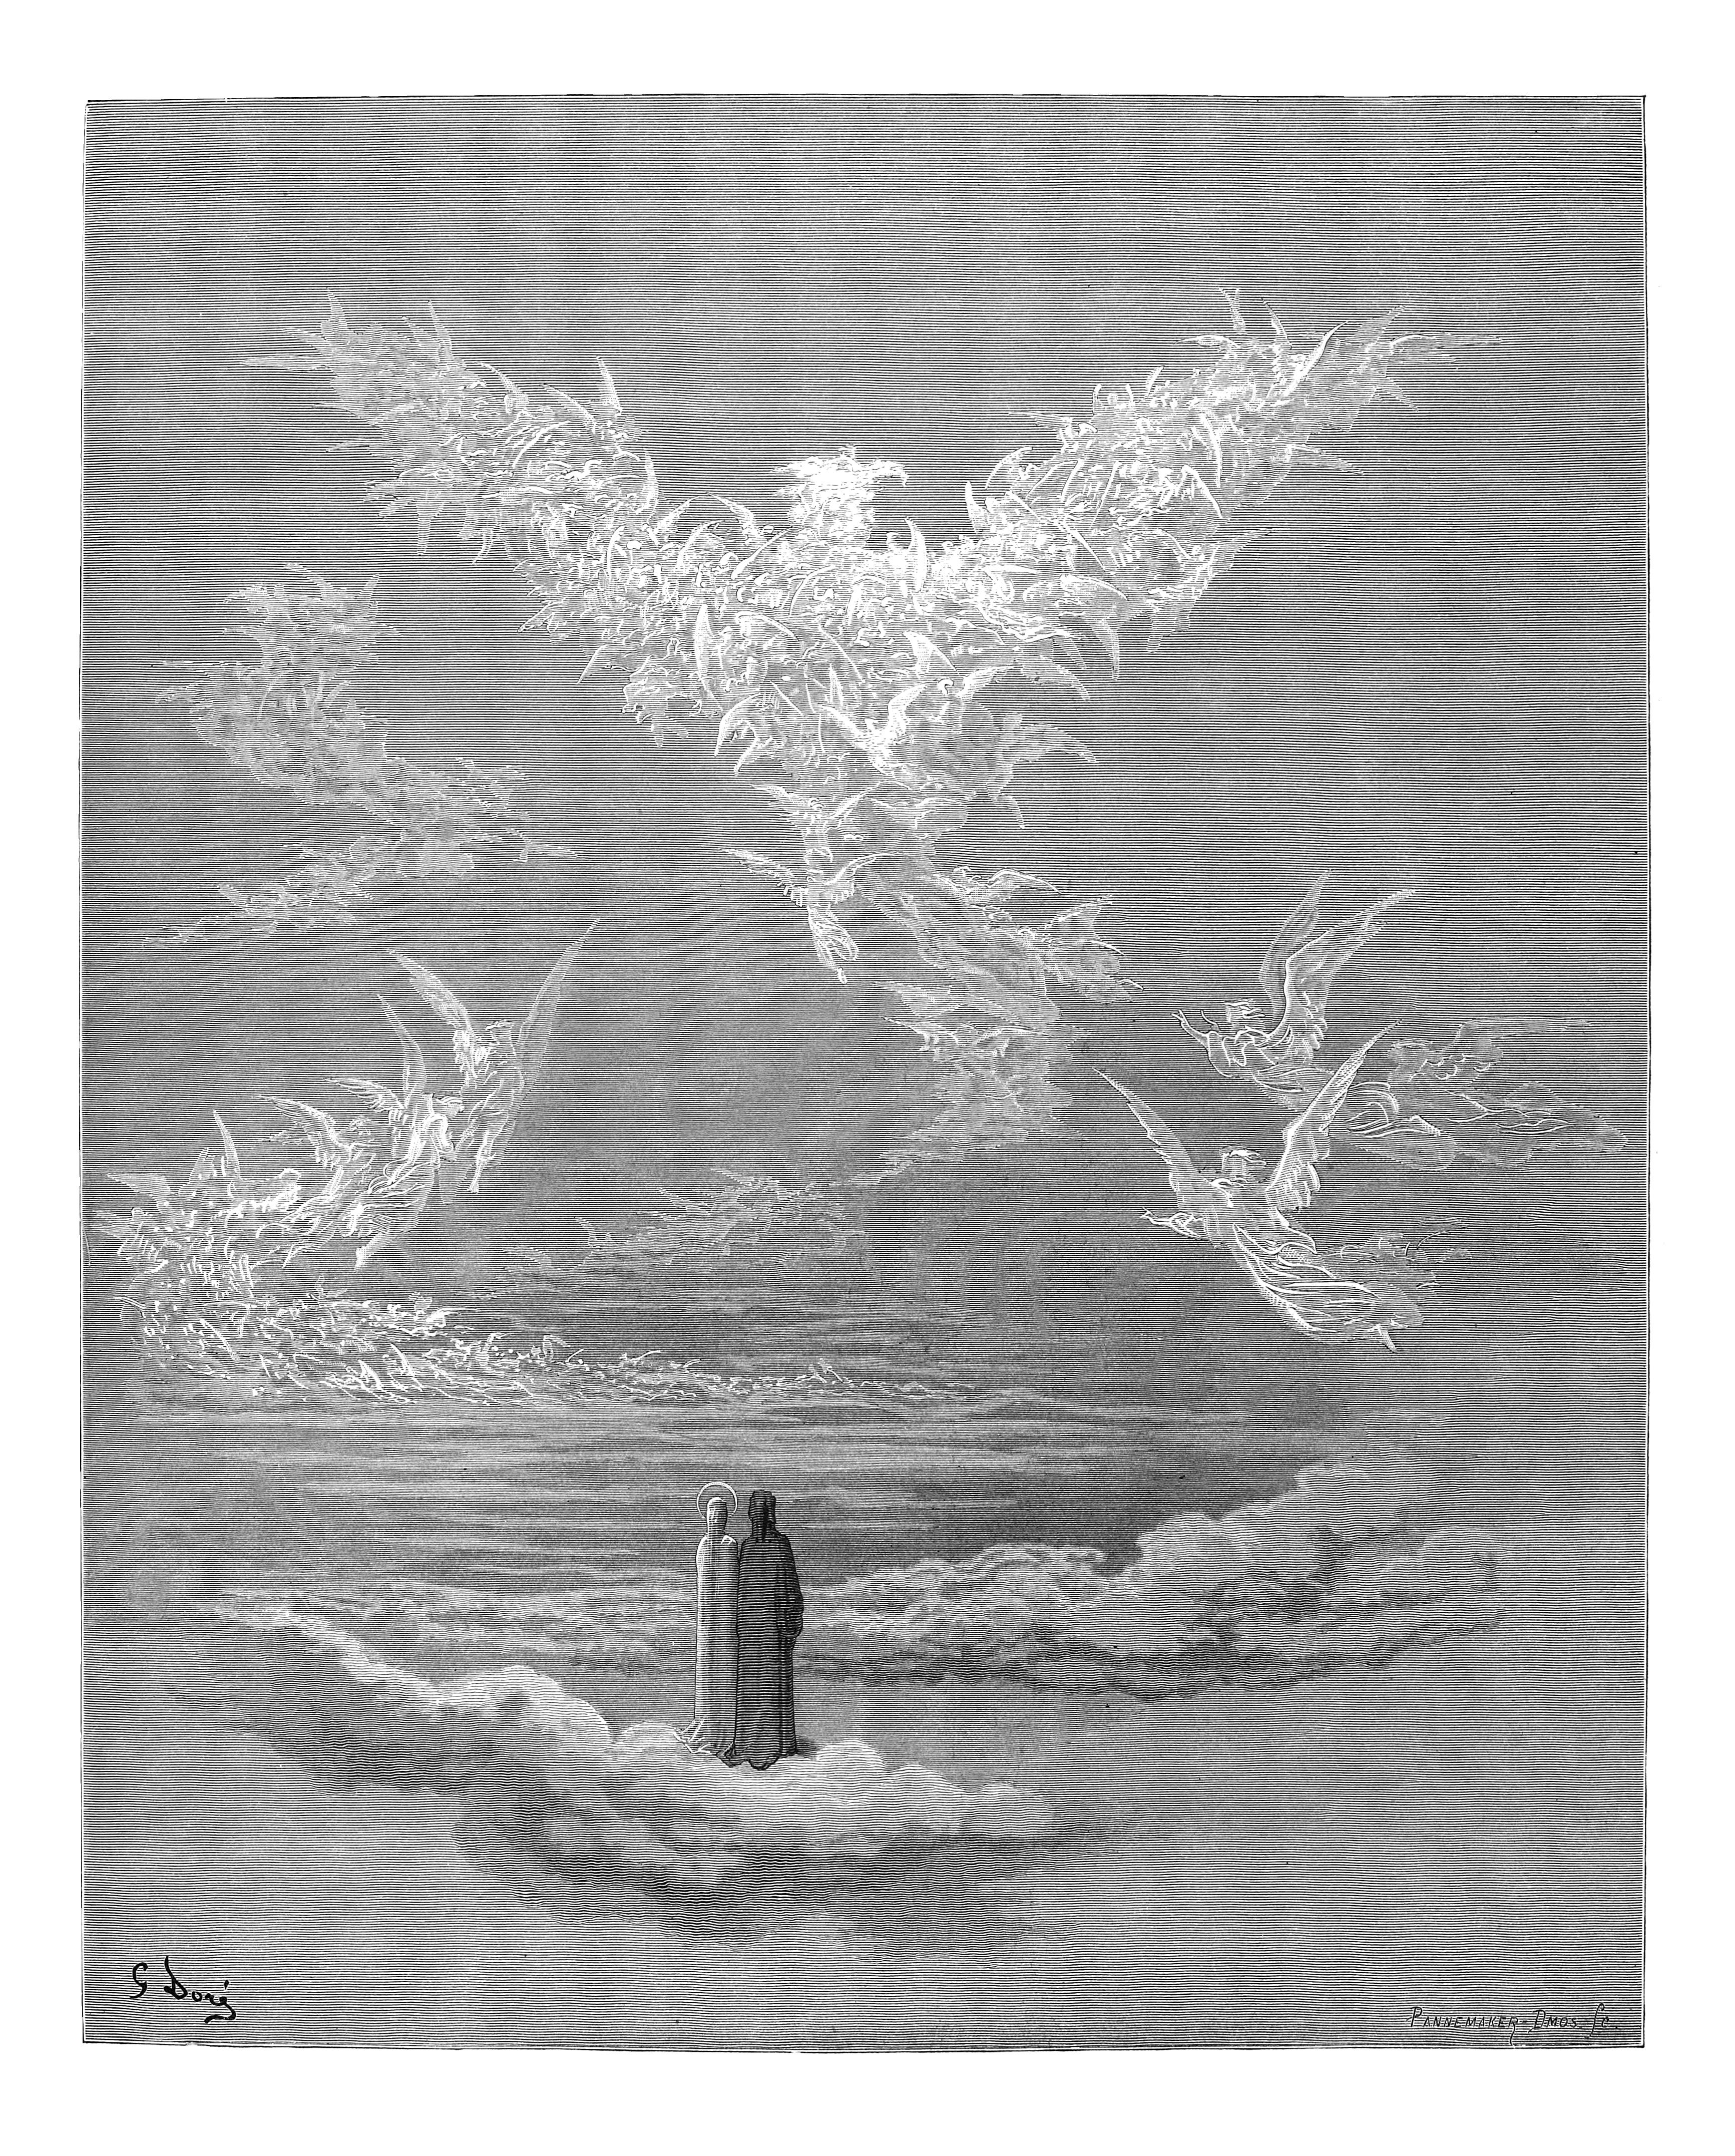
\includegraphics[height=\figsize]{illustrations/book_3/V03, c19.jpg}
\end{figure}

\begin{center}
\begin{minipage}{0.8\linewidth}
\textit{\\
"Parea dinanzi a me con l’ali aperte\\la bella image che nel dolce frui\\liete facevan l’anime conserte;"} \\
—V03, c19 \\~\\
\textit{"Before my sight appear'd, with open wings,\\The beauteous image, in fruition sweet\\Gladdening the thronged spirits. …"} \\
—B03, c19
\end{minipage}
\end{center}

\newpage

\section{Canto 20}

\begin{figure}[ht]
\centering
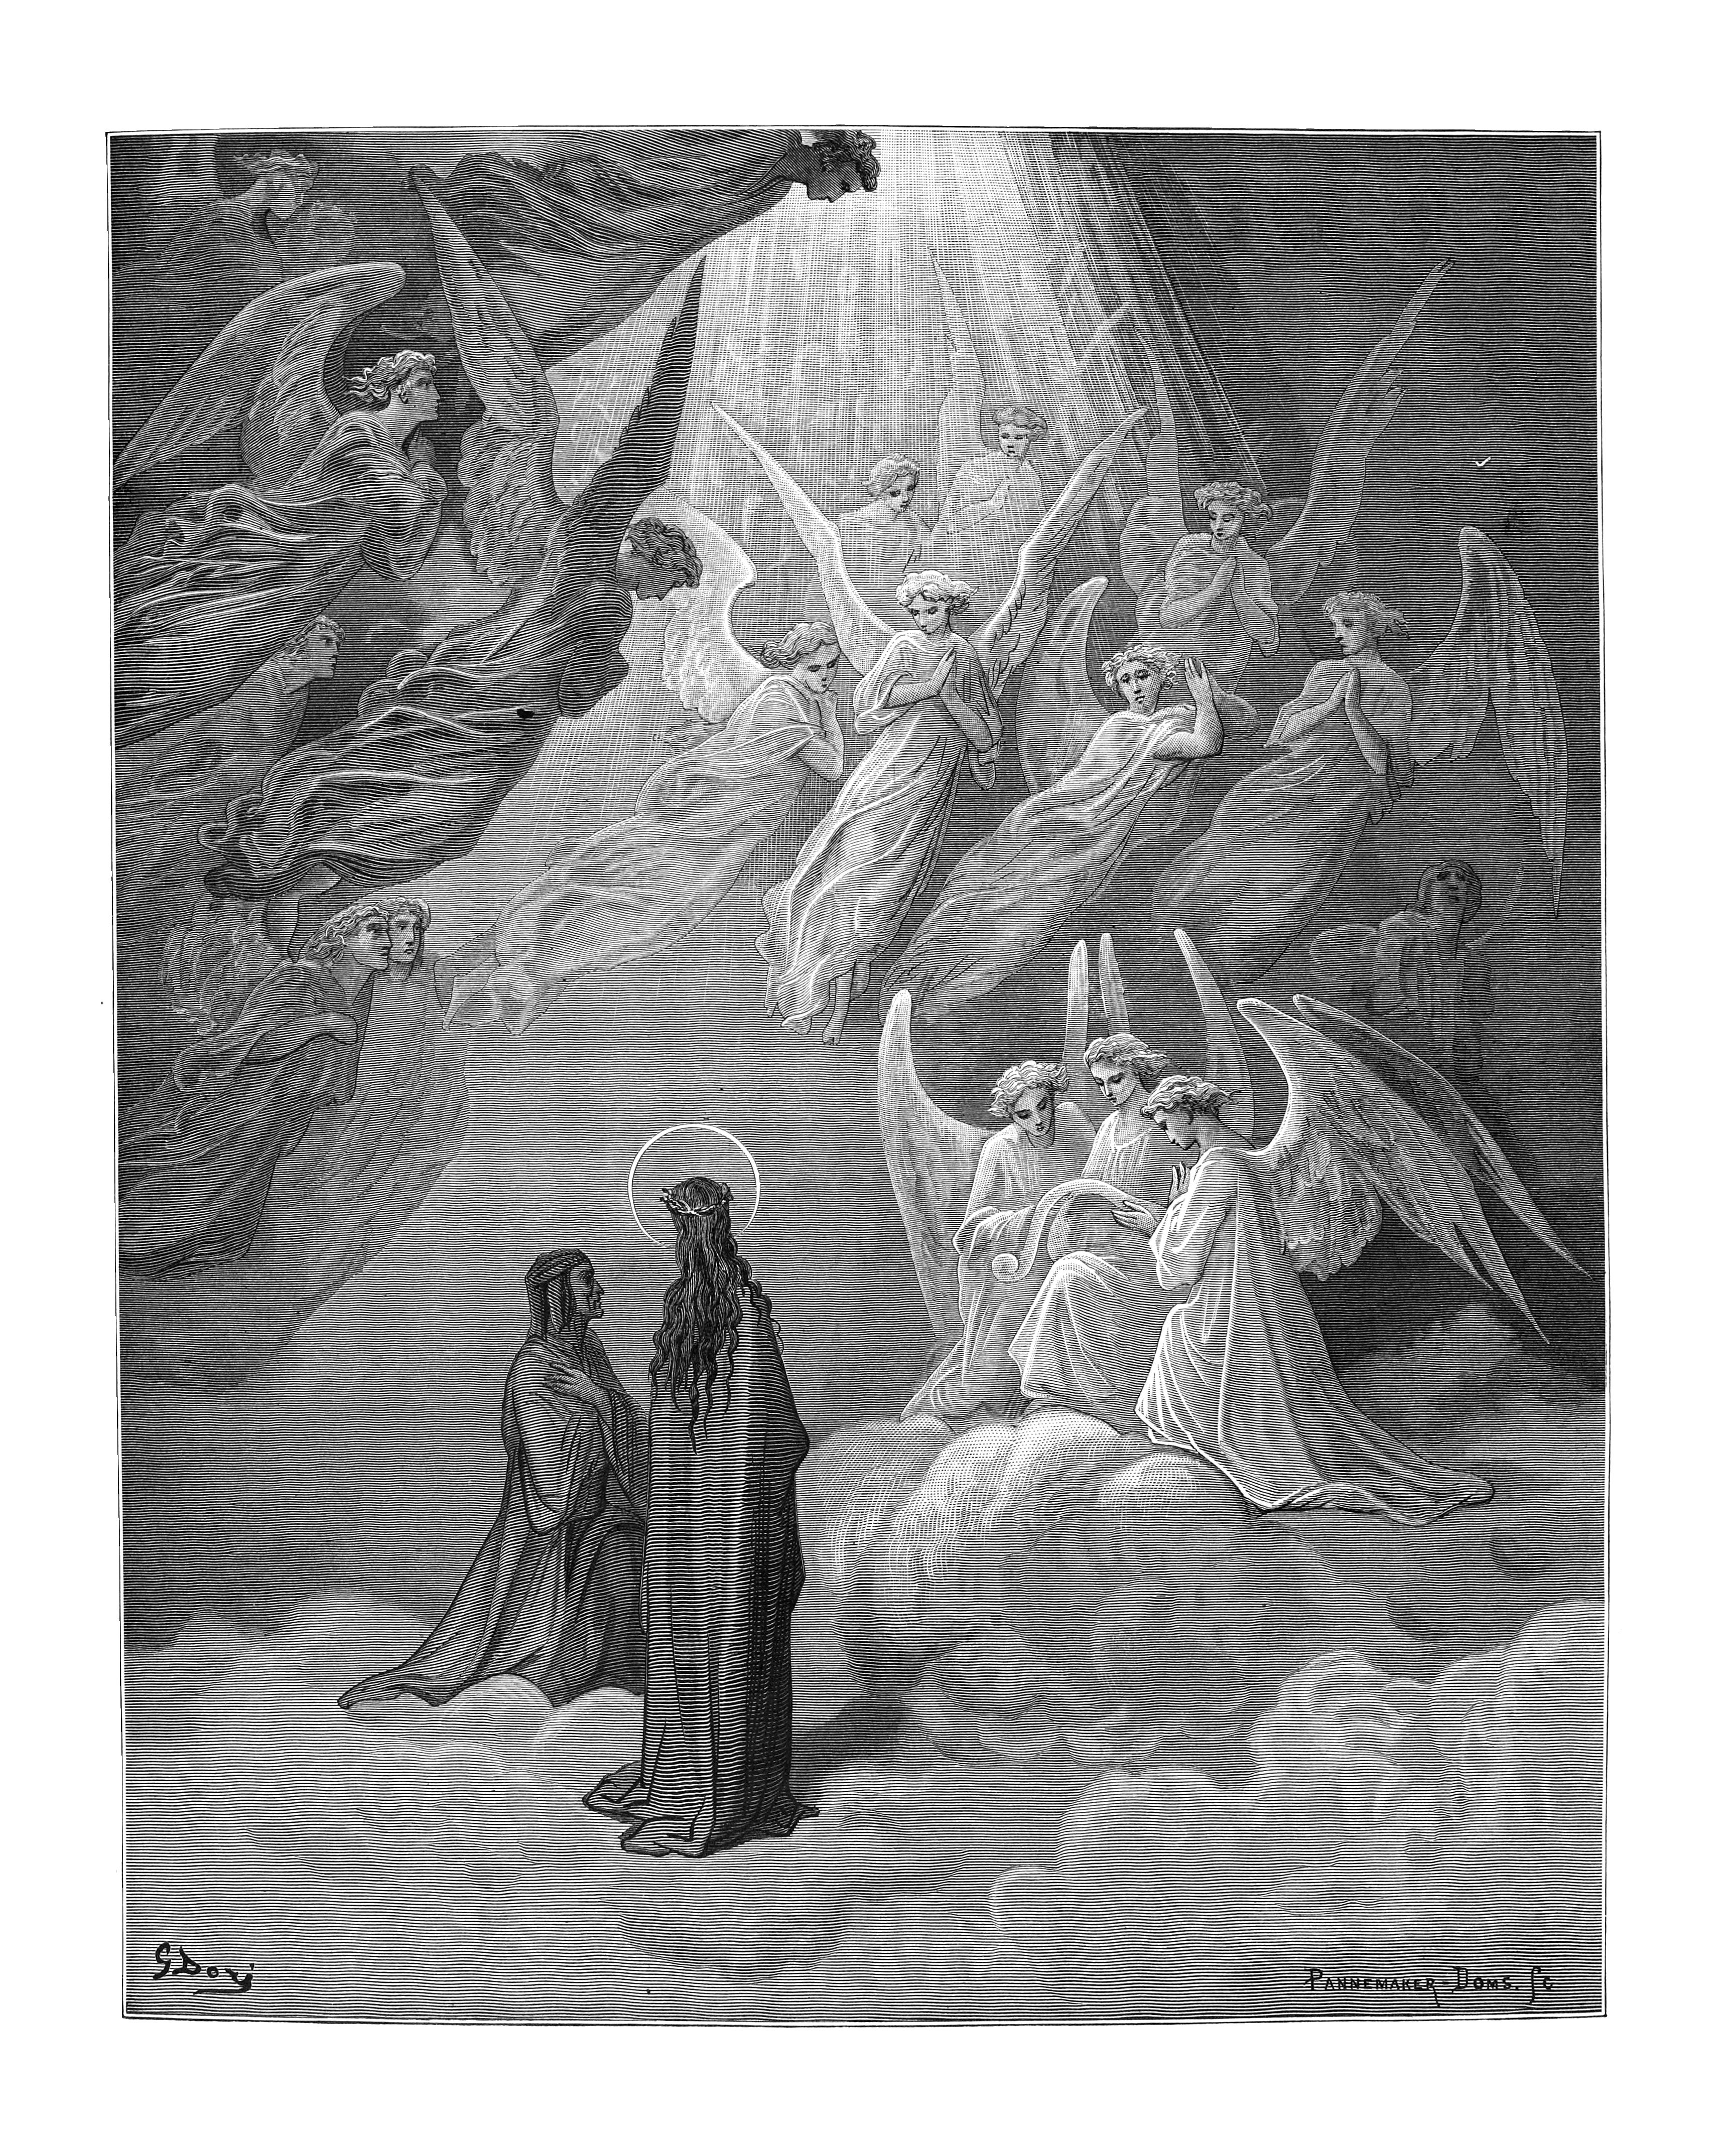
\includegraphics[height=\figsize]{illustrations/book_3/V03, c20.jpg}
\end{figure}

\begin{center}
\begin{minipage}{0.8\linewidth}
\textit{\\
"tal mi sembi\`o l’imago de la ’mprenta\\de l’etterno piacere, al cui disio\\ciascuna cosa qual ell’è diventa."} \\
—V03, c20 \\~\\
\textit{"...such appear'd\\That image stampt by the' everlasting pleasure,\\Which fashions like itself all lovely things."} \\
—B03, c20
\end{minipage}
\end{center}

\newpage

\section{Canto 21(1)}

\begin{figure}[ht]
\centering
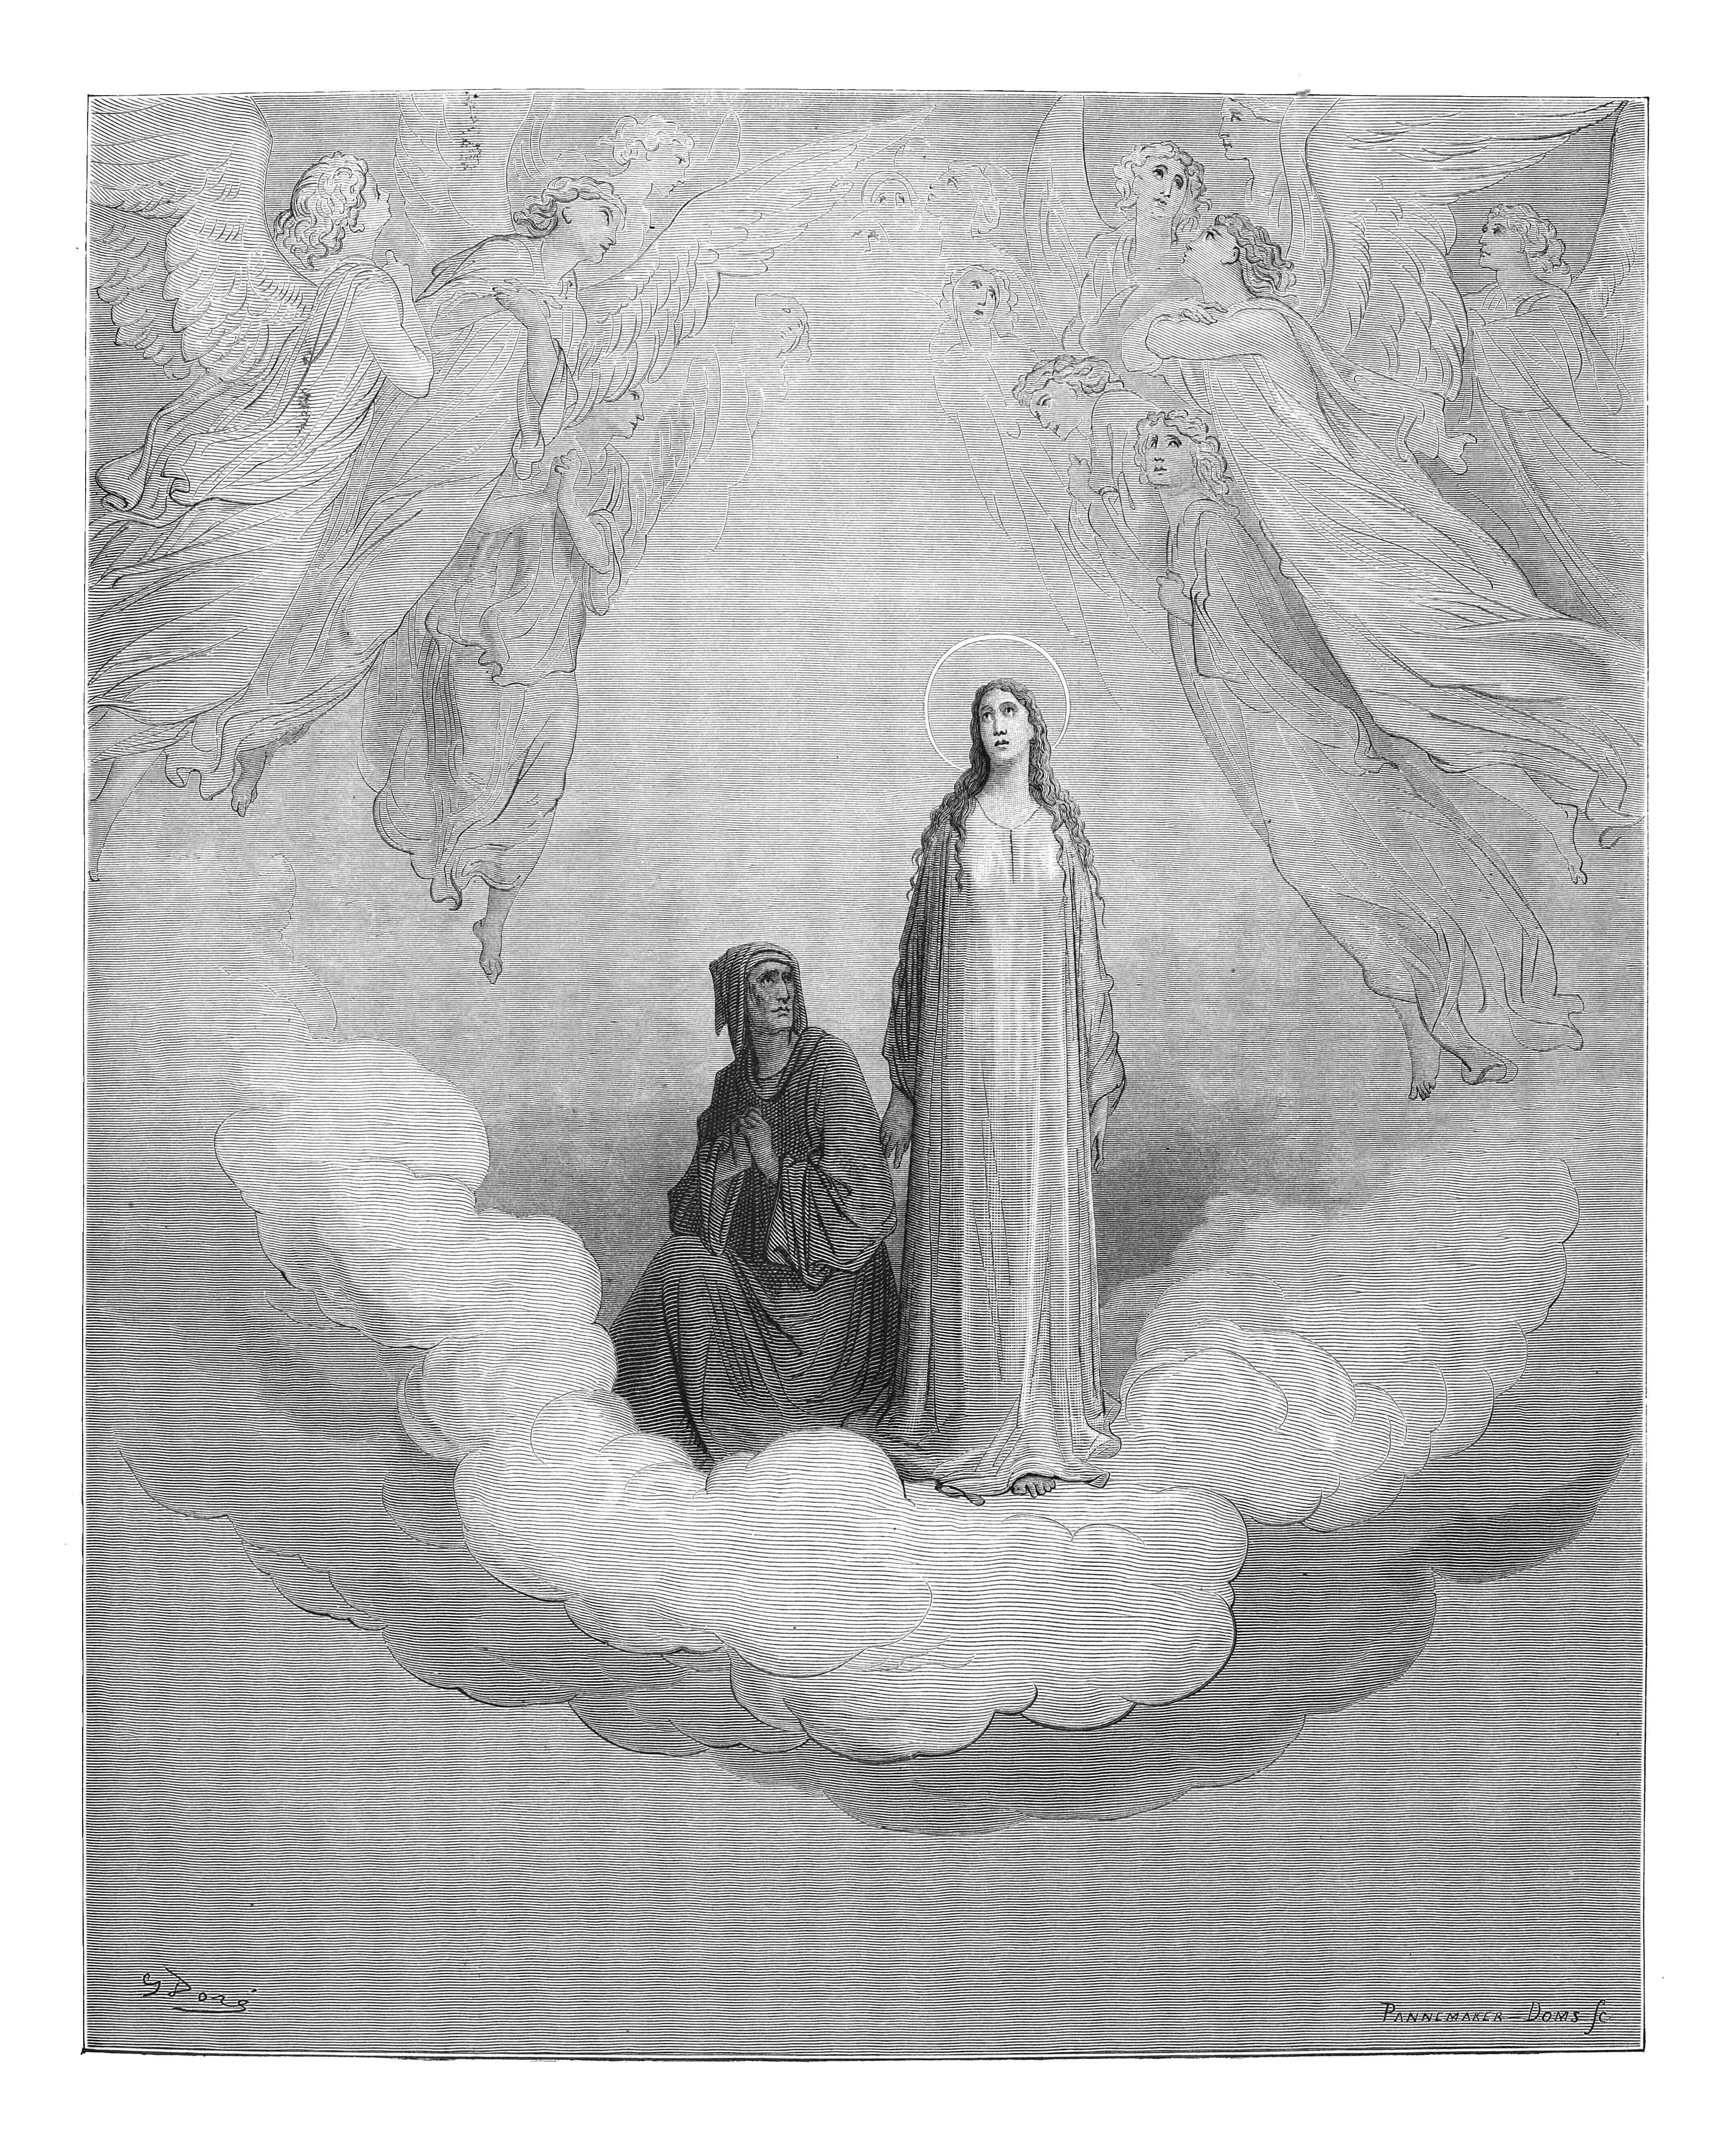
\includegraphics[height=\figsize]{illustrations/book_3/V03, c21(1).jpg}
\end{figure}

\begin{center}
\begin{minipage}{0.8\linewidth}
\textit{\\
"Già eran li occhi miei rifissi al volto\\de la mia donna, e l’animo con essi,\\e da ogne altro intento s’era tolto."} \\
—V03, c21(1) \\~\\
\textit{"Again mine eyes were fix'd on Beatrice,\\And with mine eyes my soul, that in her looks\\Found all contentment. …"} \\
—B03, c21(1)
\end{minipage}
\end{center}

\newpage

\section{Canto 21(2)}

\begin{figure}[ht]
\centering
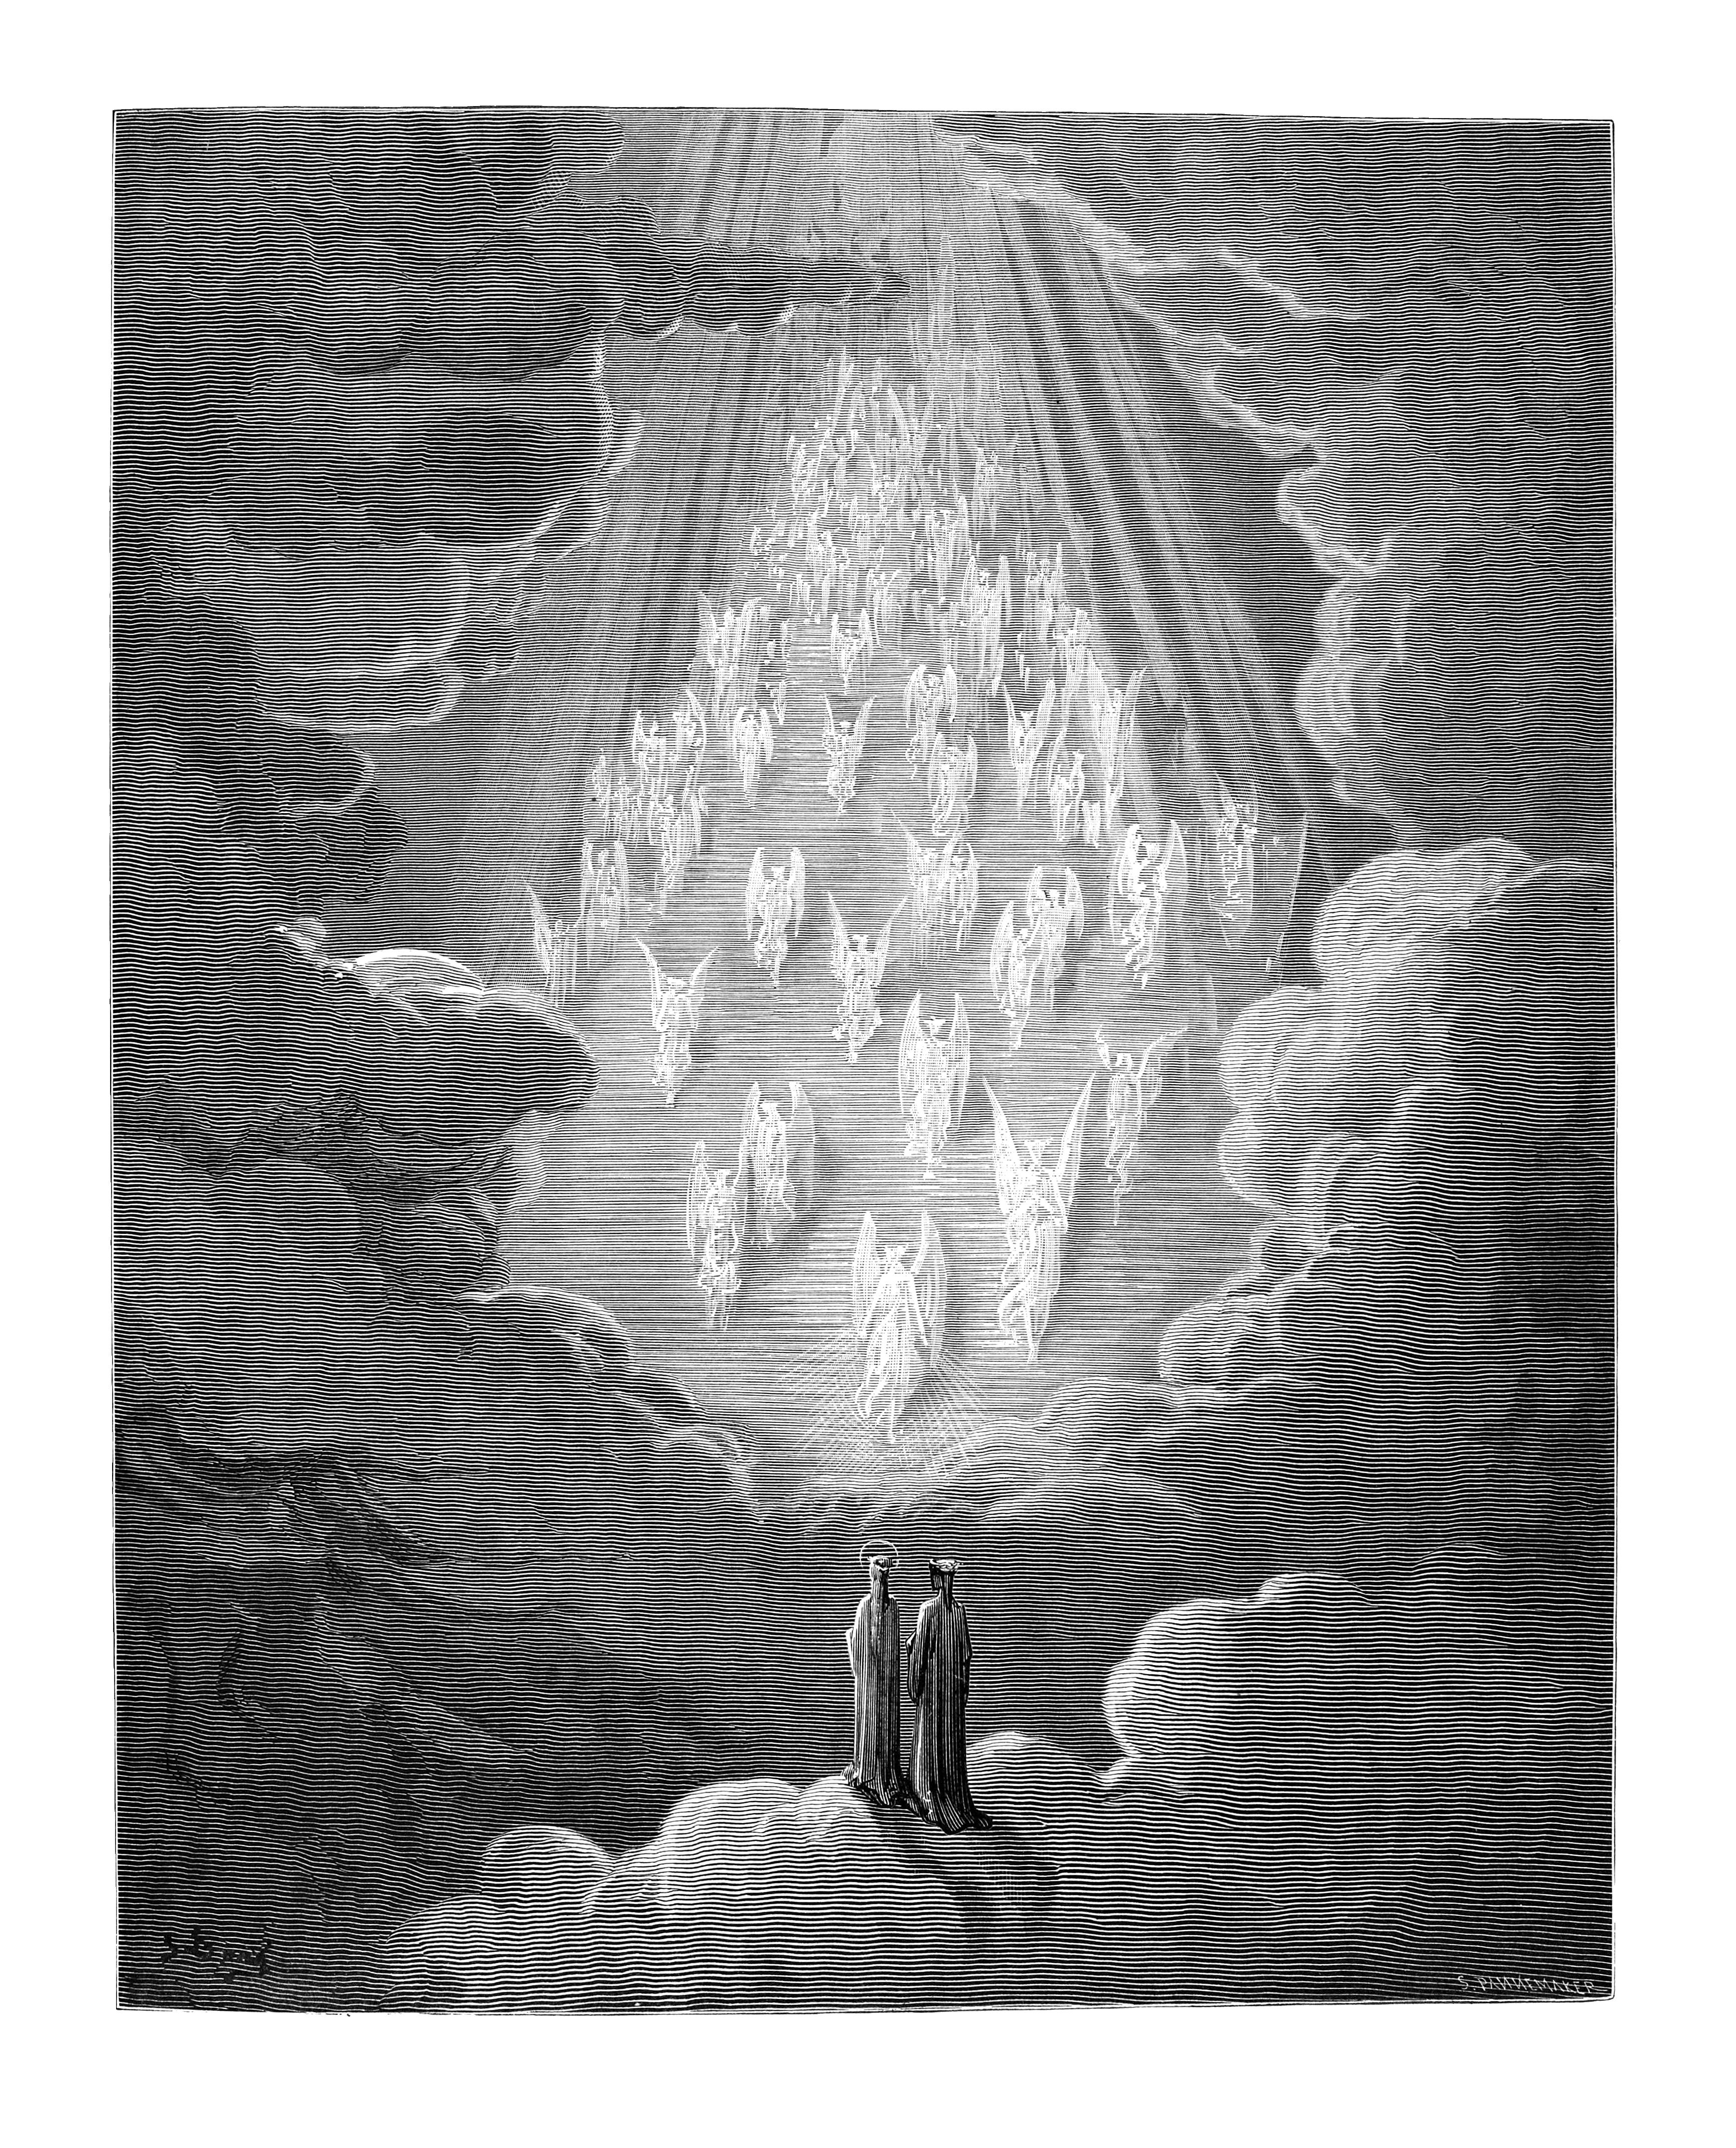
\includegraphics[height=\figsize]{illustrations/book_3/V03, c21(2).jpg}
\end{figure}

\begin{center}
\begin{minipage}{0.8\linewidth}
\textit{\\
"di color d’oro in che raggio traluce\\vid’io uno scaleo eretto in suso\\tanto, che nol seguiva la mia luce."} \\
—V03, c21(2) \\~\\
\textit{"...I saw rear'd up,\\In colour like to sun-illumin'd gold.\\A ladder, which my ken pursued in vain,\\So lofty was the summit; ..."} \\
—B03, c21(2)
\end{minipage}
\end{center}

\newpage

\section{Canto 26}

\begin{figure}[ht]
\centering
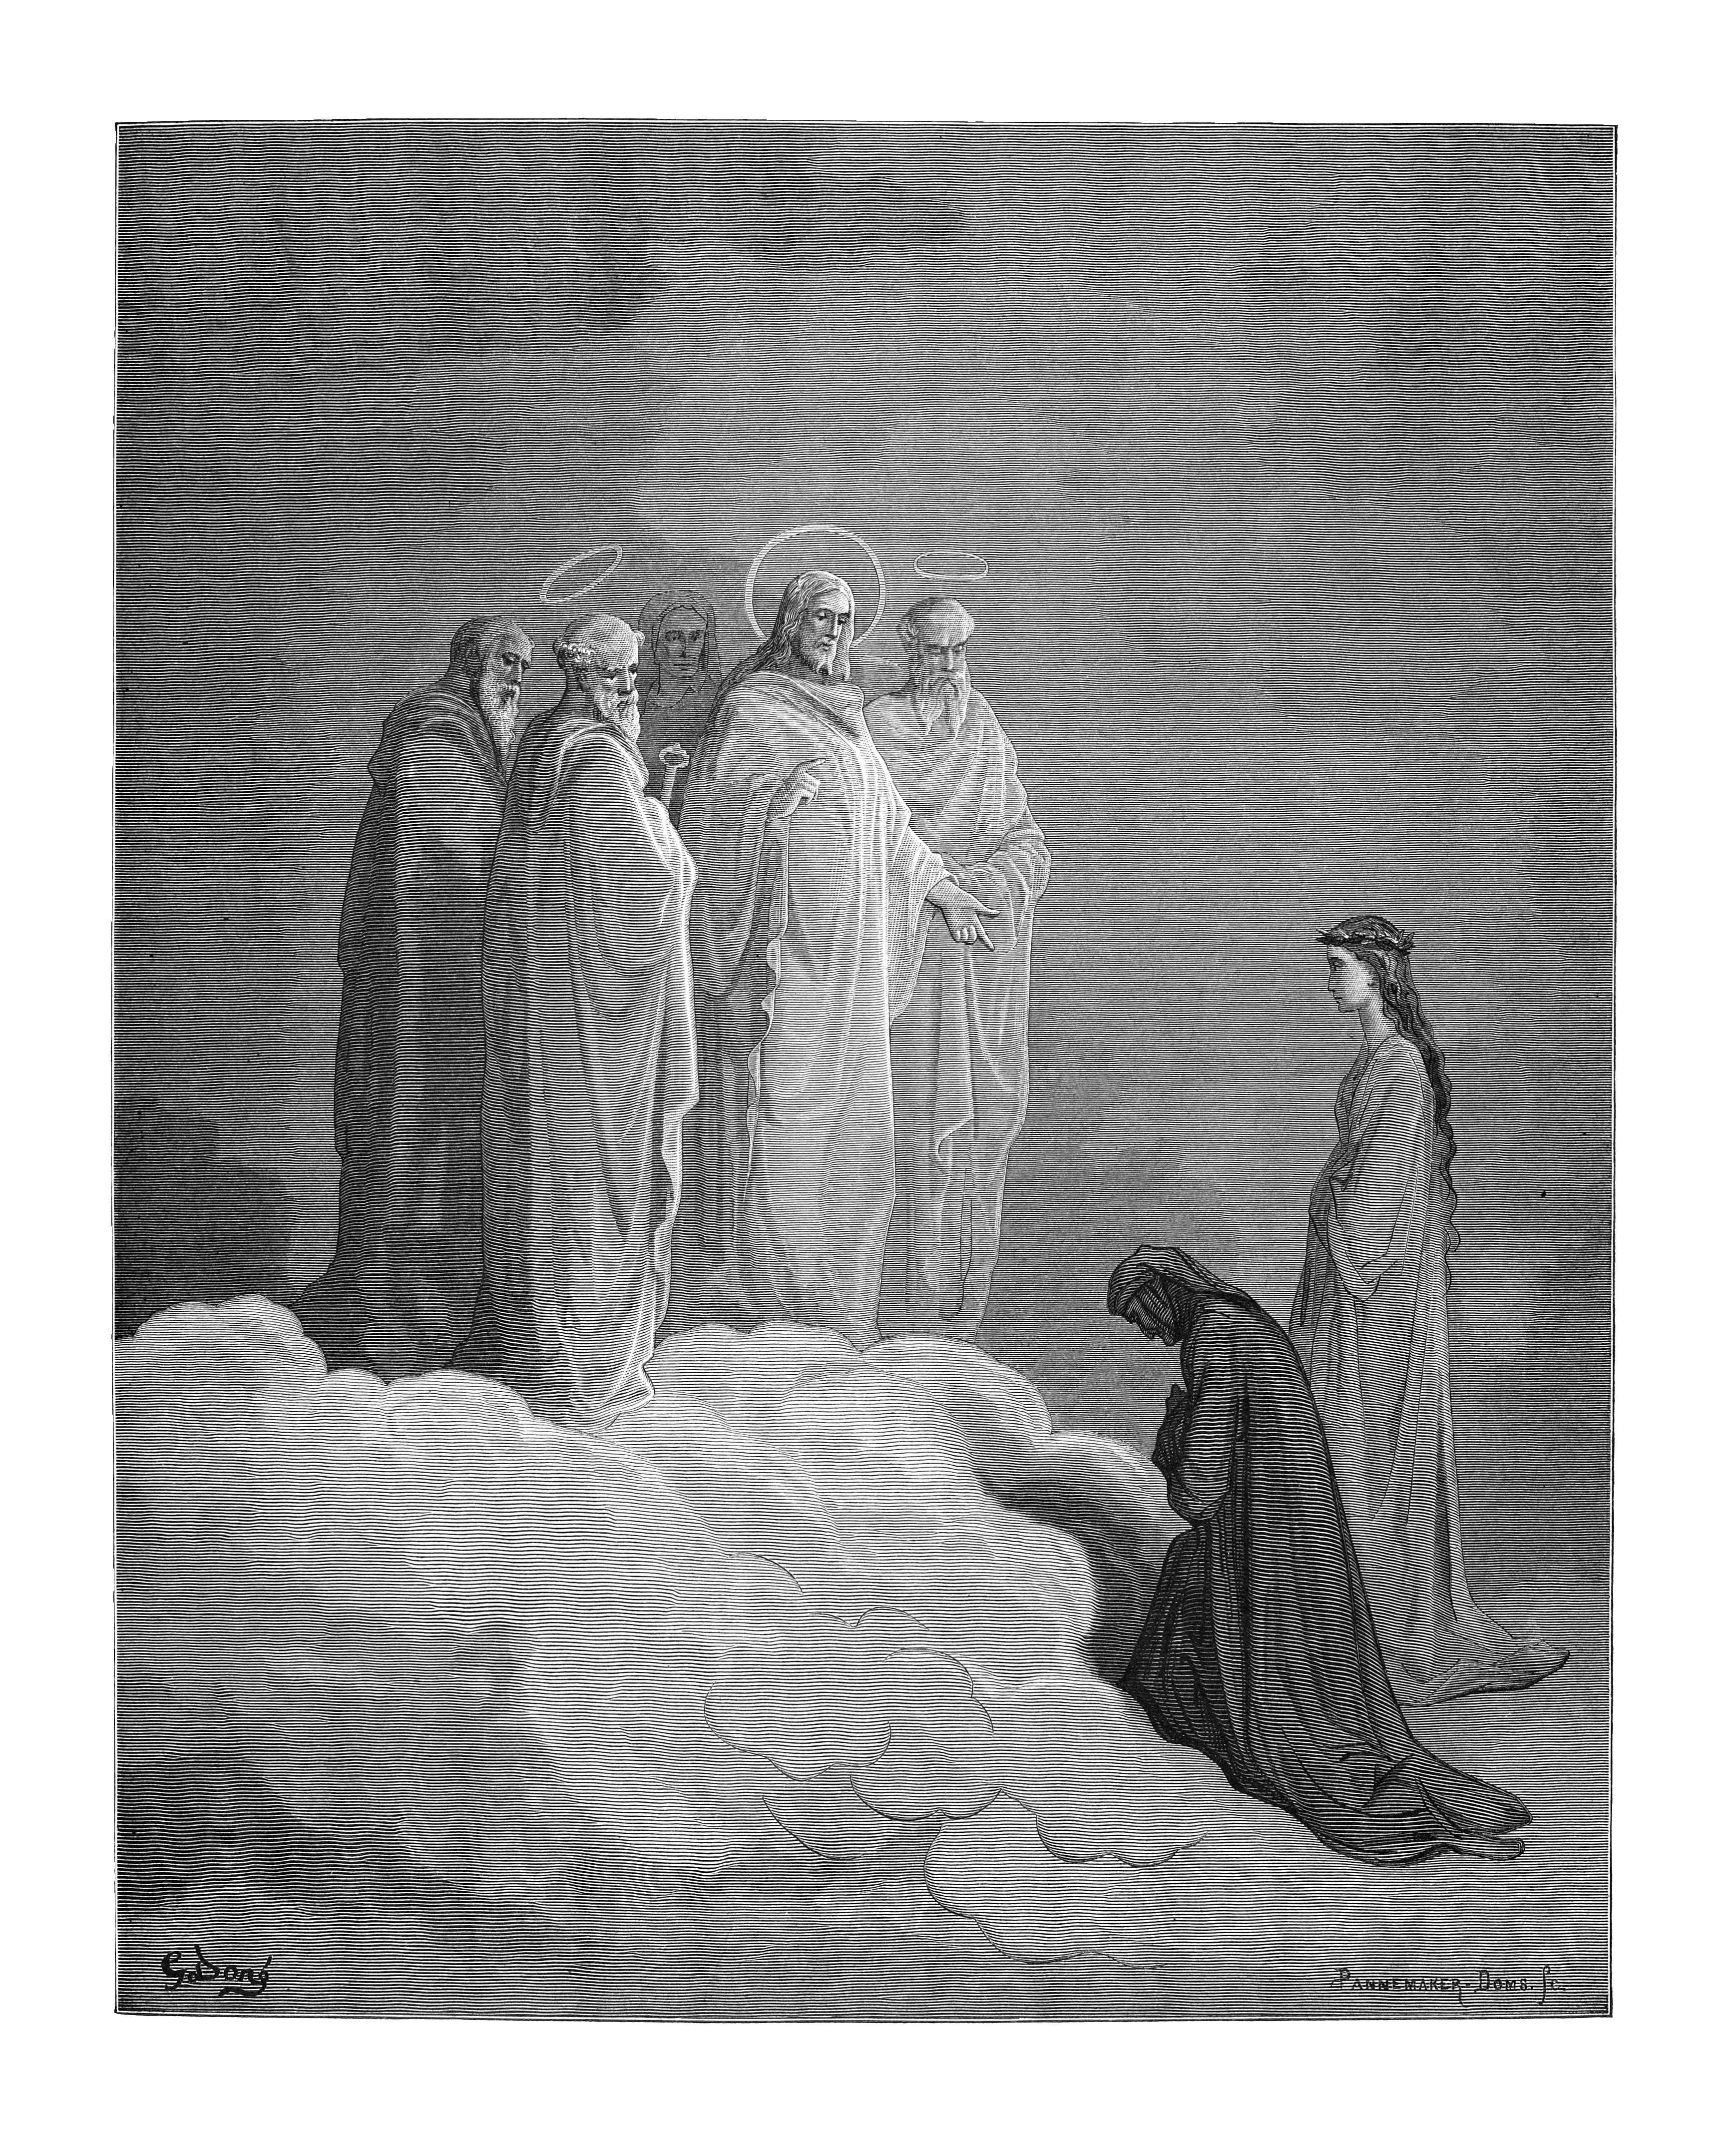
\includegraphics[height=\figsize]{illustrations/book_3/V03, c26.jpg}
\end{figure}

\begin{center}
\begin{minipage}{0.8\linewidth}
\textit{\\
"Comincia dunque; e di’ ove s’appunta\\l’anima tua, …"} \\
—V03, c26 \\~\\
\textit{"...Say then,\\Beginning, to what point thy soul aspires:"} \\
—B03, c26
\end{minipage}
\end{center}

\newpage

\section{Canto 27}

\begin{figure}[ht]
\centering
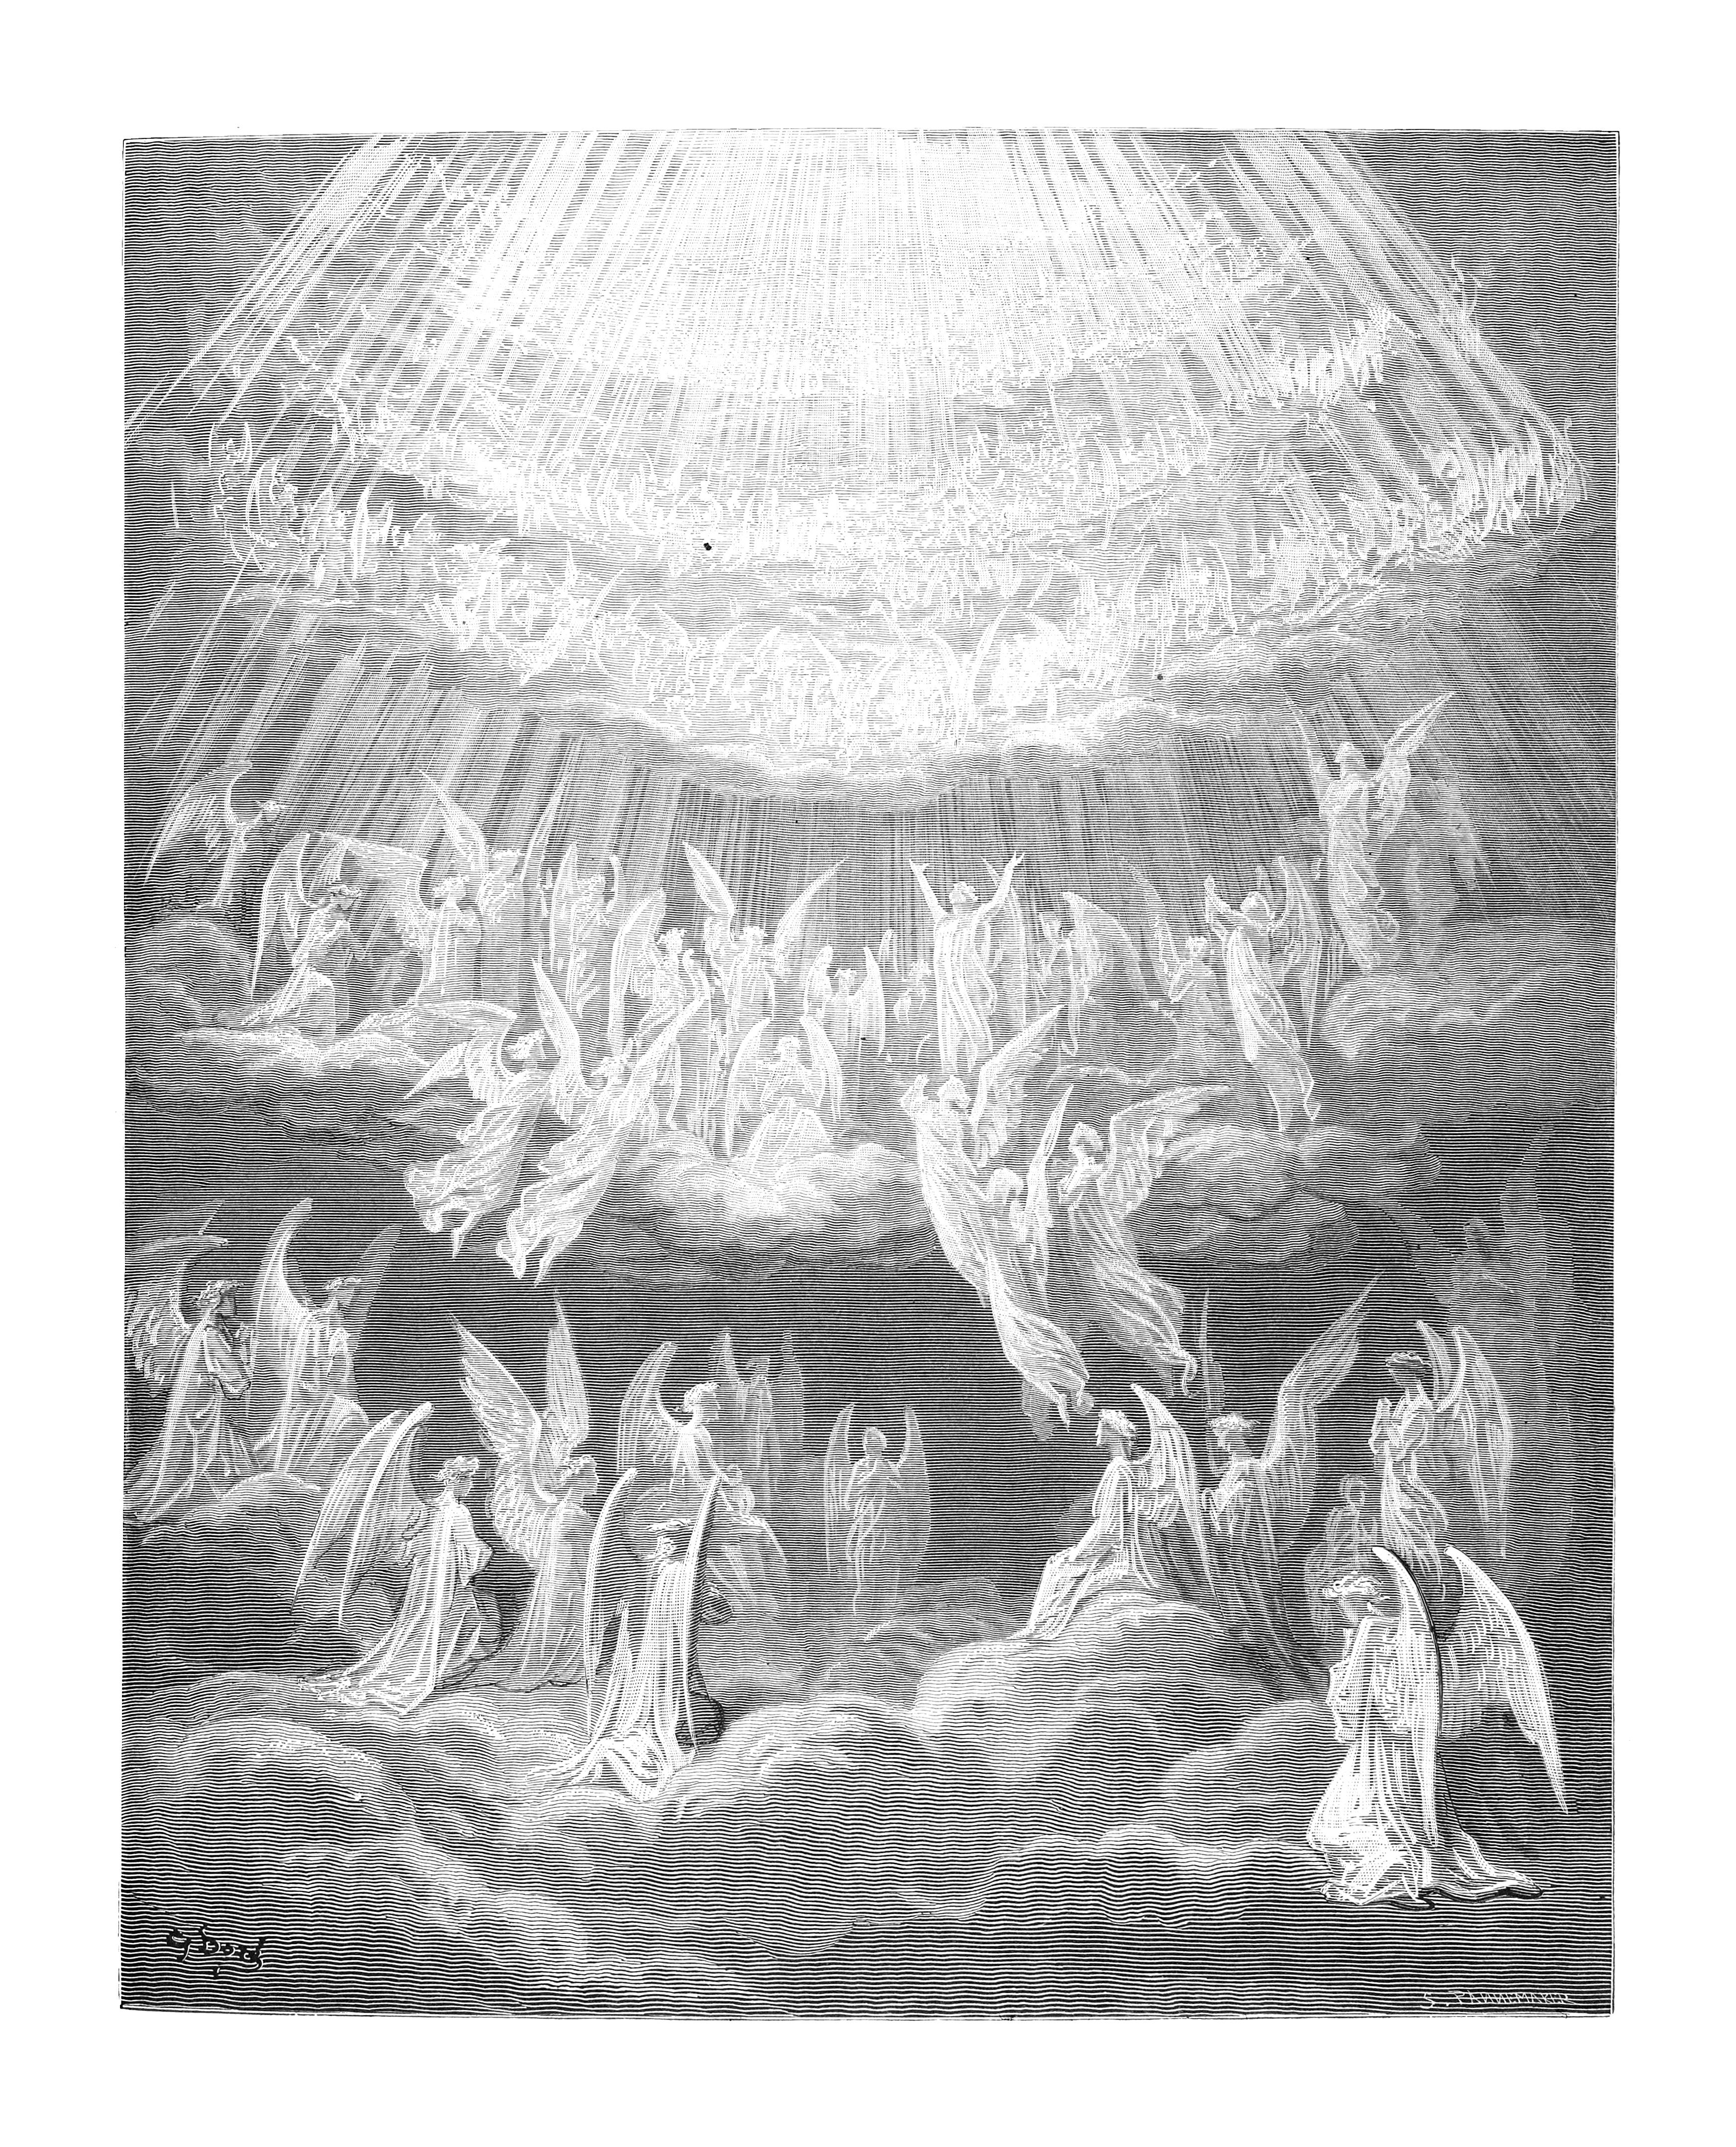
\includegraphics[height=\figsize]{illustrations/book_3/V03, c27.jpg}
\end{figure}

\begin{center}
\begin{minipage}{0.8\linewidth}
\textit{\\
"...m’inebriava il dolce canto.\\Ci\`o ch’io vedeva mi sembiava un riso\\de l’universo; per che mia ebbrezza\\intrava per l’udire e per lo viso."} \\
—V03, c27 \\~\\
\textit{"...with the song\\My spirit reel'd, so passing sweet the strain:\\And what I saw was equal ecstasy;"} \\
—B03, c27
\end{minipage}
\end{center}

\newpage

\section{Canto 28}

\begin{figure}[ht]
\centering
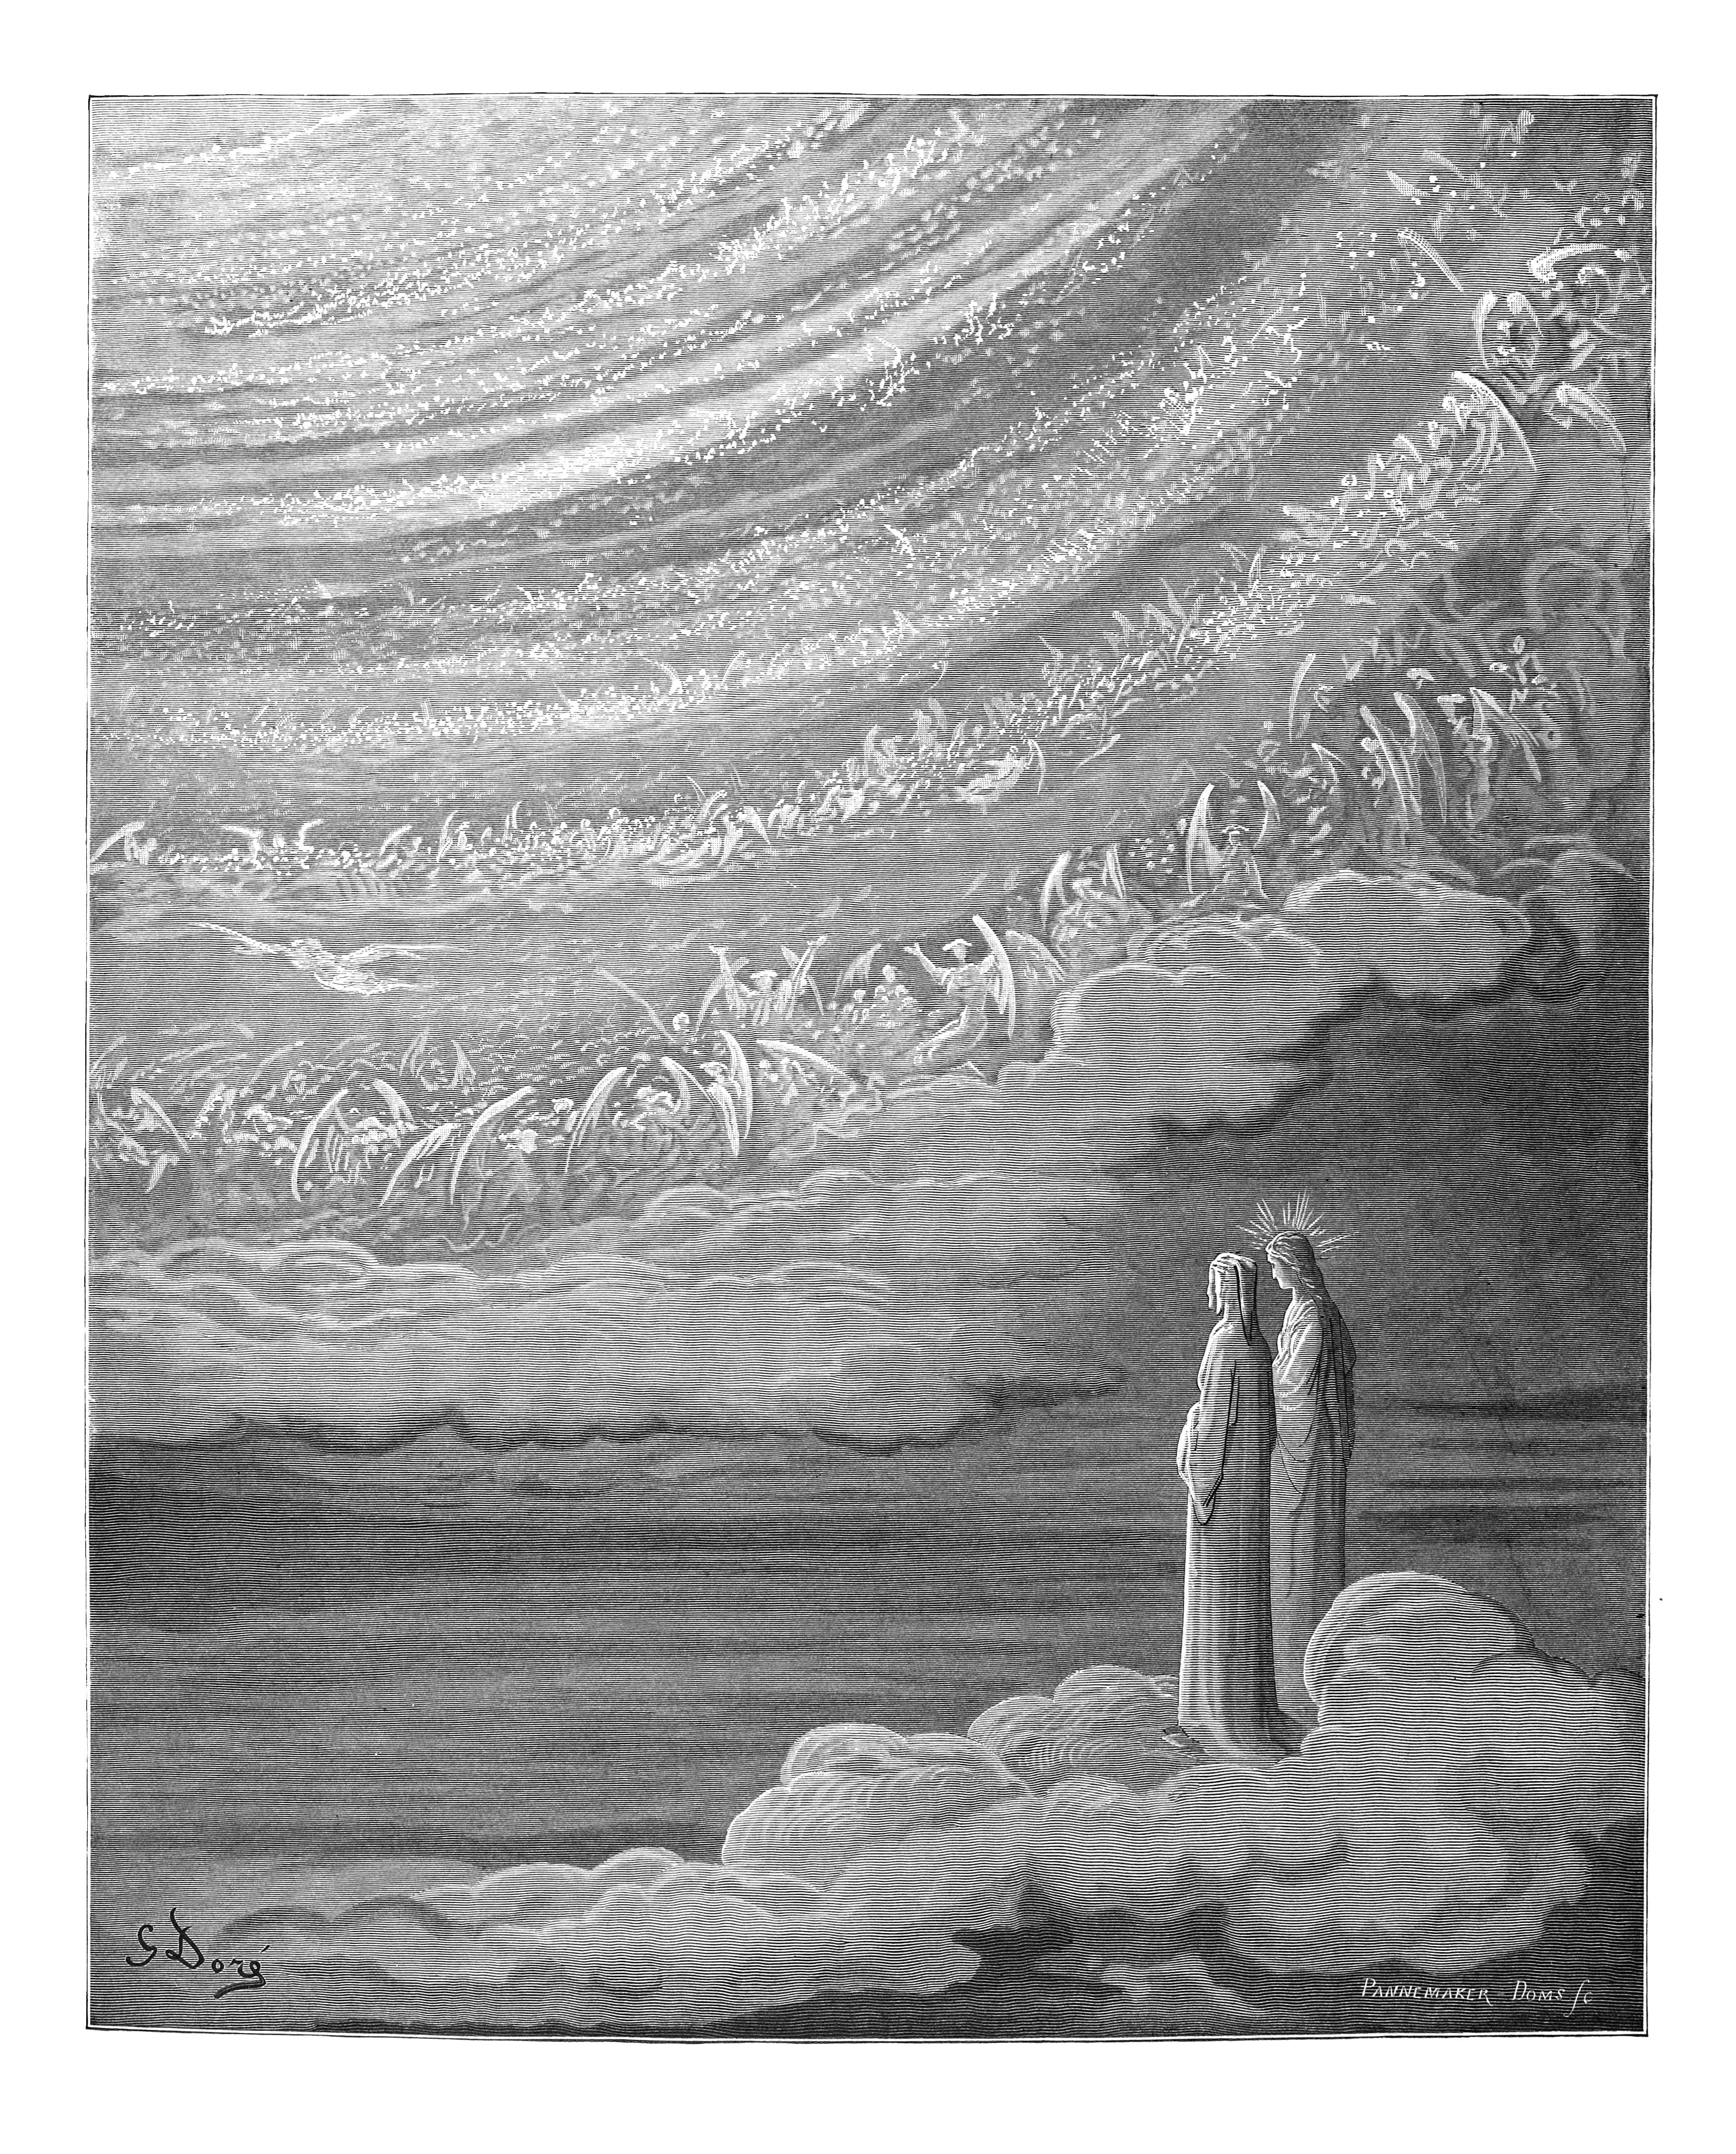
\includegraphics[height=\figsize]{illustrations/book_3/V03, c28.jpg}
\end{figure}

\begin{center}
\begin{minipage}{0.8\linewidth}
\textit{\\
"L’incendio suo seguiva ogne scintilla;\\ed eran tante, che ’l numero loro\\più che ’l doppiar de li scacchi s’inmilla."} \\
—V03, c28 \\~\\
\textit{"...every sparkle shivering to new blaze,\\In number did outmillion the account\\Reduplicate upon the chequer'd board."} \\
—B03, c28
\end{minipage}
\end{center}

\newpage

\section{Canto 31(1)}

\begin{figure}[ht]
\centering
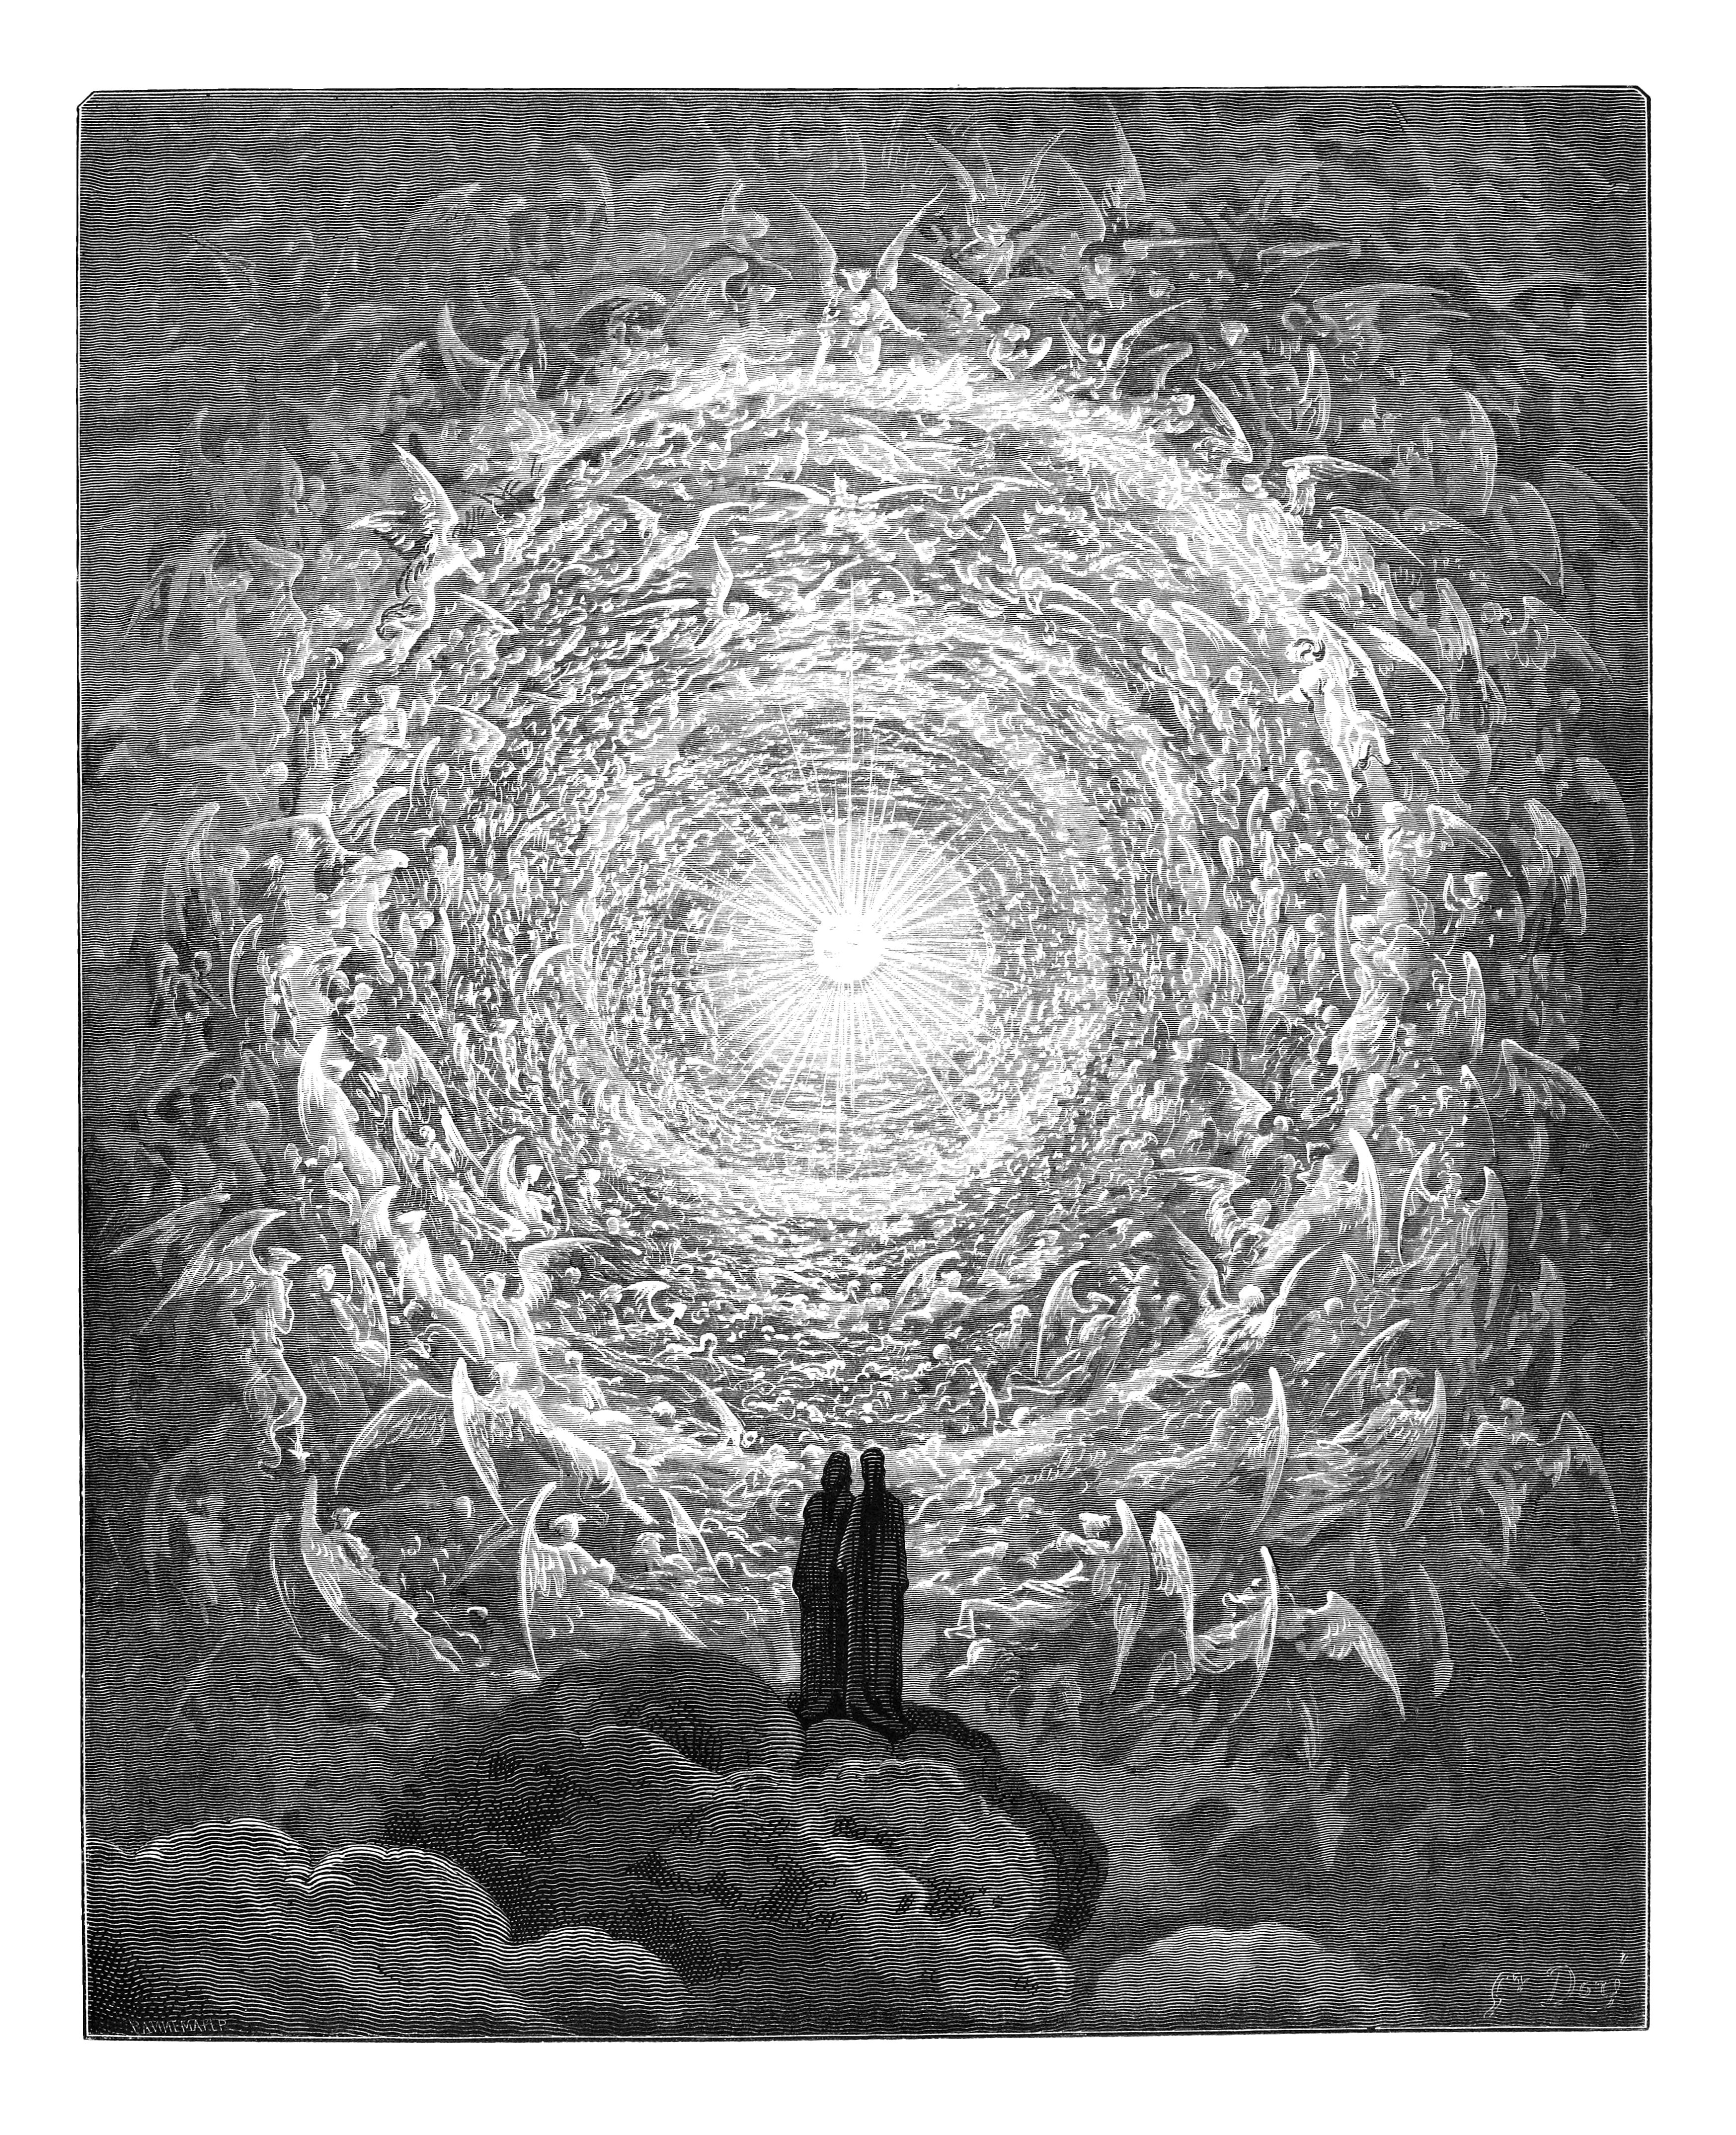
\includegraphics[height=\figsize]{illustrations/book_3/V03, c31(1).jpg}
\end{figure}

\begin{center}
\begin{minipage}{0.8\linewidth}
\textit{\\
"In forma dunque di candida rosa\\mi si mostrava la milizia santa"} \\
—V03, c31(1) \\~\\
\textit{"In fashion, as a snow-white rose, lay then\\Before my view the saintly multitude,"} \\
—B03, c31(1)
\end{minipage}
\end{center}

\newpage

\section{Canto 31(2)}

\begin{figure}[ht]
\centering
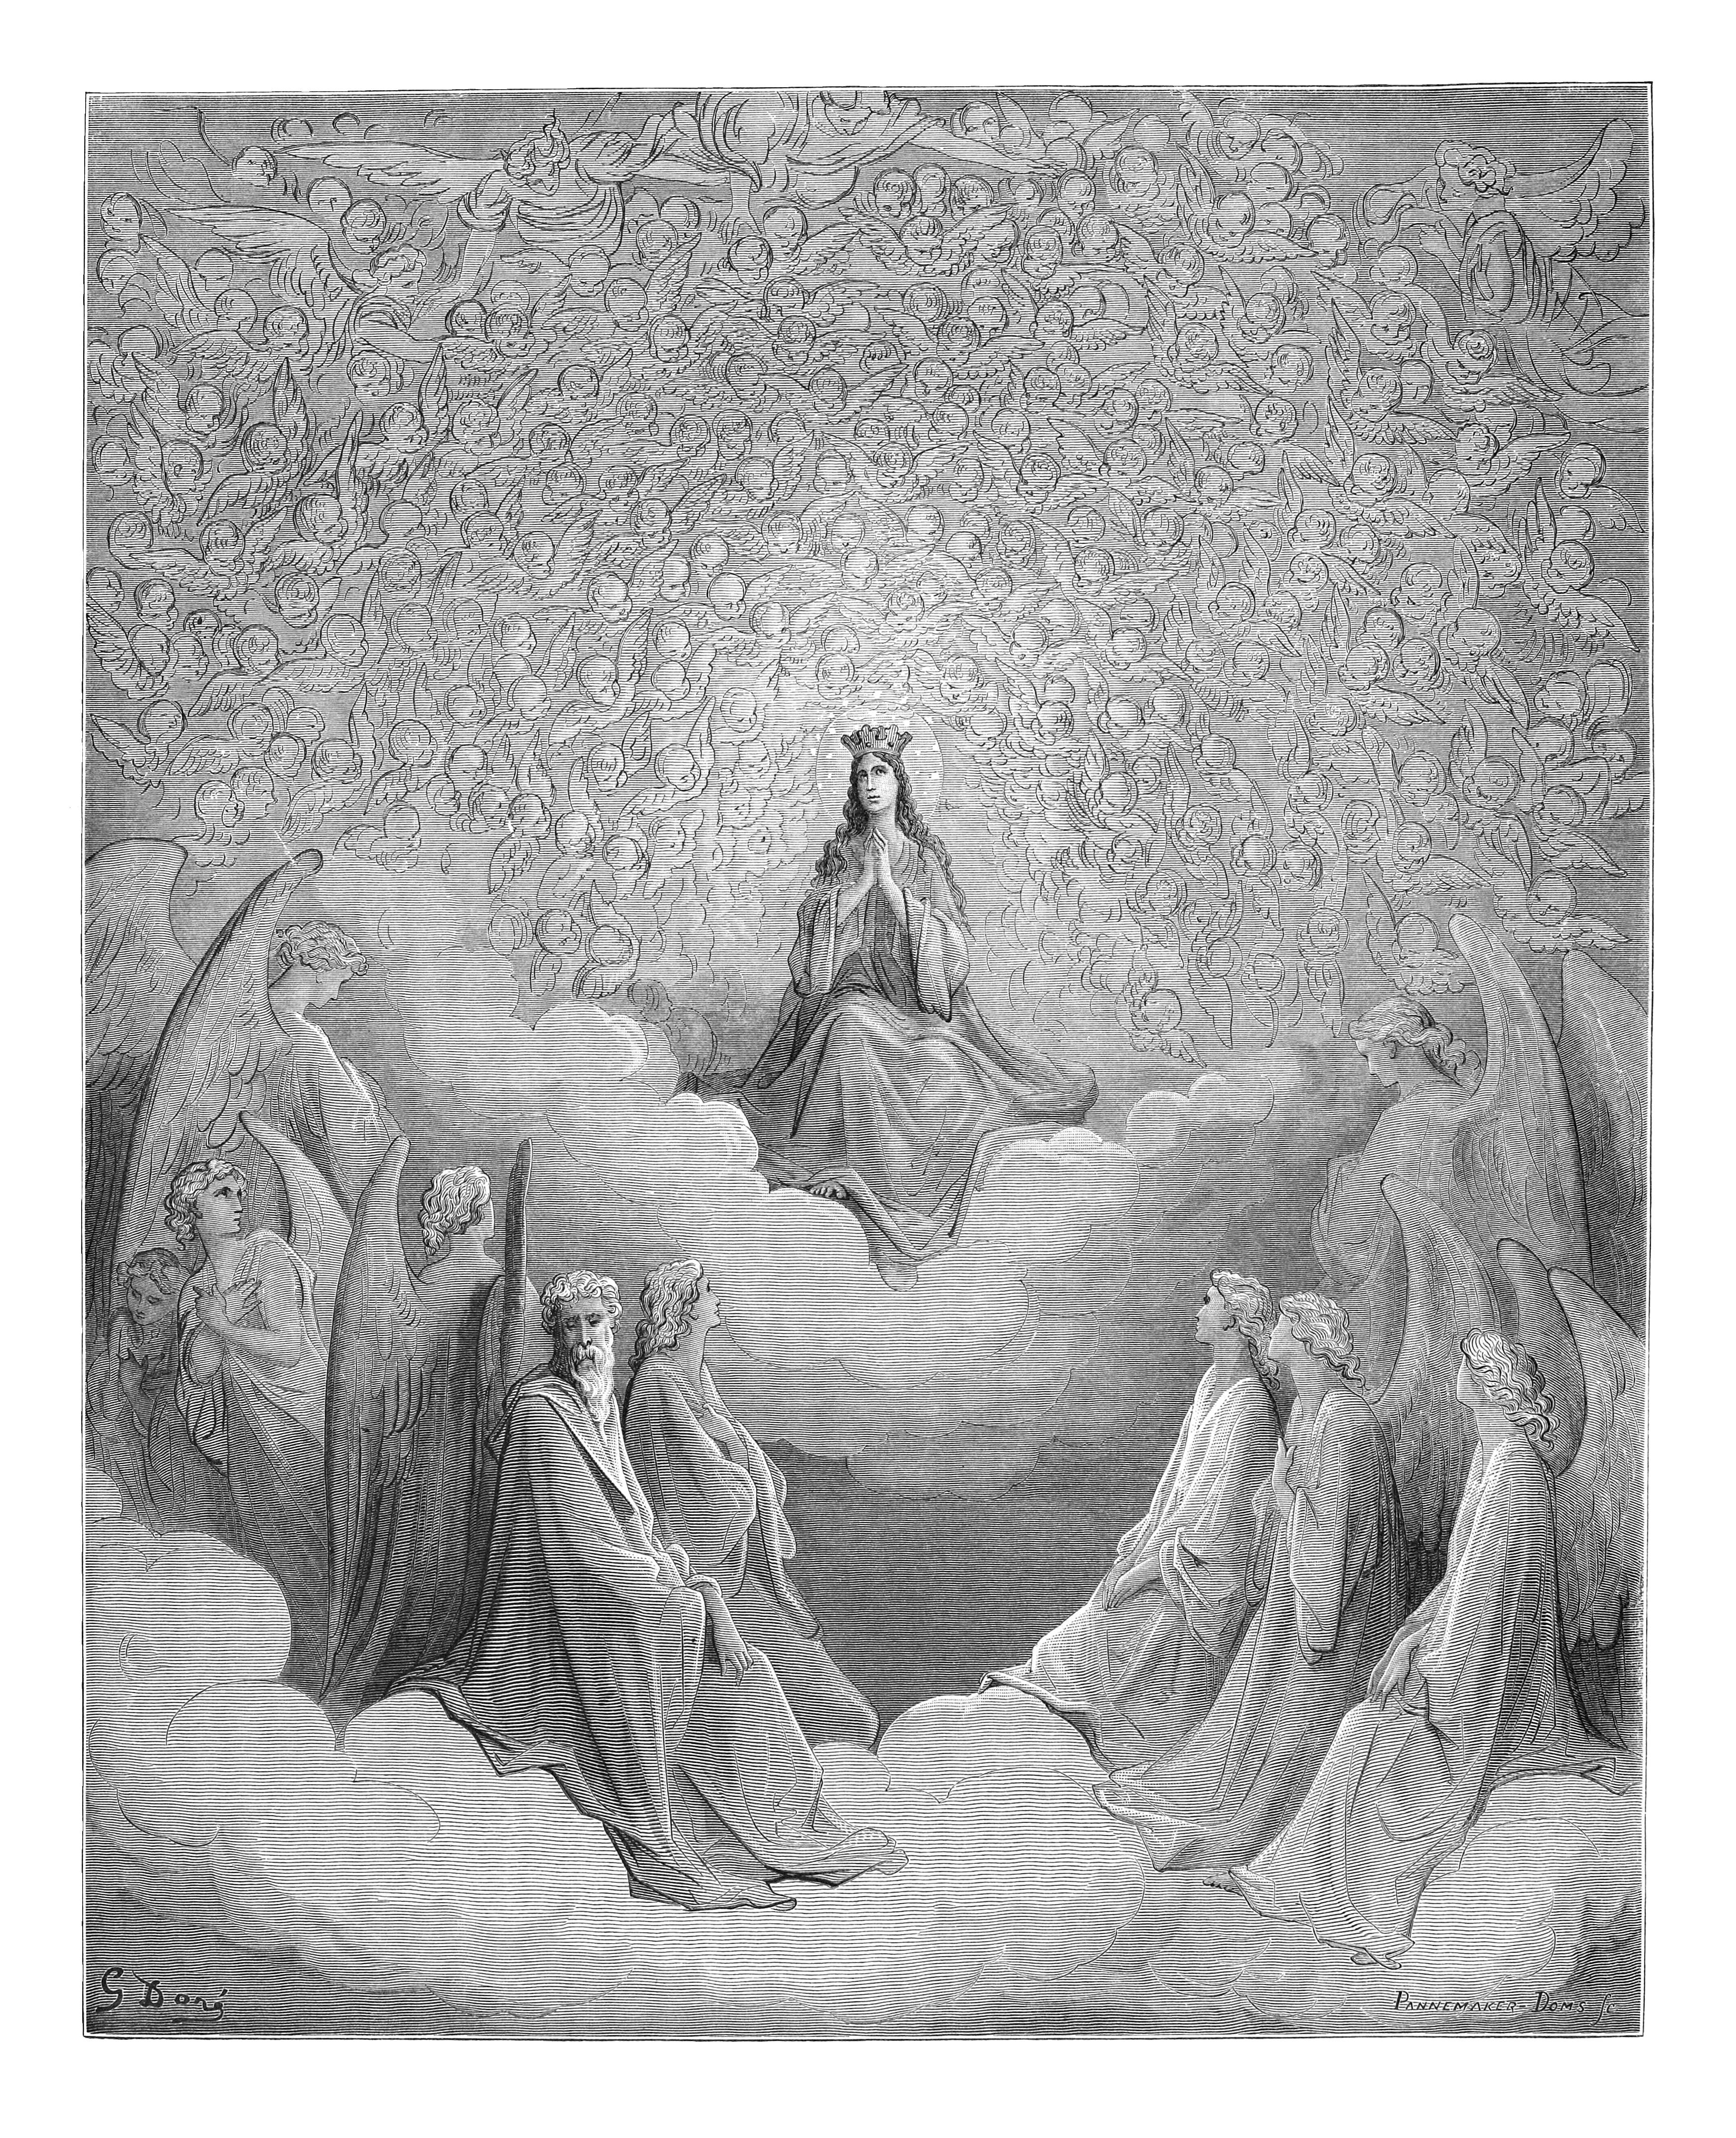
\includegraphics[height=\figsize]{illustrations/book_3/V03, c31(2).jpg}
\end{figure}

\begin{center}
\begin{minipage}{0.8\linewidth}
\textit{\\
"Vidi a lor giochi quivi e a lor canti\\ridere una bellezza, che letizia\\era ne li occhi a tutti li altri santi;"} \\
—V03, c31(2) \\~\\
\textit{"...At their glee\\And carol, smil' d the Lovely One of heav'n,\\That joy was in the eyes of all the blest."} \\
—B03, c31(2)
\end{minipage}
\end{center}

\end{document}